%%==================================================
%% diss.tex for SJTU Master Thesis
%% based on CASthesis
%% version: 0.3a
%% Encoding: UTF-8
%%==================================================

% 字号选项: c5size 五号(默认) cs4size 小四
% 双面打印(注意字号设置)
%\documentclass[cs4size, a4paper, twoside]{sjtuthesis} 
% 单面打印(注意字号设置)
 \documentclass[cs5size, a4paer, oneside, openany]{sjtuthesis} 


% \usepackage[sectionbib]{chapterbib}%每章都用参考文献
 

%%%使用算法
\usepackage{algorithm}
\usepackage{algpseudocode}
\usepackage{amsmath}
\usepackage{graphics}
\usepackage{epsfig}
\renewcommand{\algorithmicrequire}{\textbf{输入:}}
\renewcommand{\algorithmicensure}{\textbf{输出:}}
\renewcommand{\algorithmcfname}{算法}
\floatname{algorithm}{算法}
%%%end of 使用算法

\newboolean{DOIT}
\setboolean{DOIT}{false}%编译某些只想自己看的内容,编译true,否则false

%% 行距缩放因子(x倍字号)
\renewcommand{\baselinestretch}{1.3}

% 设置图形文件的搜索路径
\graphicspath{{figure/}{figures/}{logo/}{logos/}{graph/}{graphs}}

%%========================================
%% 在sjtuthesis.cls中定义的有用命令
%%========================================
% \cndash 中文破折号
% 数学常量
% \me 对数常数e
% \mi 虚数单位i
% \mj 虚数单位j
% \dif 直立的微分算符d为直立体。
% 可伸长的数学箭头、等号
% \myRightarrow{}{}
% \myLeftarrow{}{}
% \myBioarrow{}{}
% \myLongEqual{}{}
% 参考文献
% \upcite{} 上标引用
%%========================================


\begin{document}

%%%%%%%%%%%%%%%%%%%%%%%%%%%%%% 
%% 封面
%%%%%%%%%%%%%%%%%%%%%%%%%%%%%% 

% 中文封面内容(关注内容而不是形式)
\title{社交网络中部分信息缺失条件下的社区发现}
\author{李奇平}
\advisor{王灿,陈英}
\degree{学士}
\defenddate{2013年6月1日}
\school{上海交通大学}
\institute{计算机科学与技术}
\studentnumber{5090209296}
\major{专业名称}

% 英文封面内容(关注内容而不是表现形式)
\englishtitle{Community Detection in Incomplete Social Networks}
\englishauthor{\textsc{Qiping Li}}
\englishadvisor{A.P \textsc{Can Wang}, A.P \textsc{Ying Chen}}
\englishschool{Shanghai Jiao Tong University}
\englishinstitute{\textsc{Depart of Computer Science and Technology} \\
  \textsc{Shanghai Jiao Tong University} \\
  \textsc{Shanghai, P.R.China}}
\englishdegree{Bachelor}
\englishmajor{Computer Science}
\englishdate{June. 1st, 2013}

% 封面
\maketitle

% 英文封面
\makeenglishtitle

% 论文原创性声明和使用授权
\makeDeclareOriginal
\makeDeclareAuthorization

%%%%%%%%%%%%%%%%%%%%%%%%%%%%%% 
%% 前言
%%%%%%%%%%%%%%%%%%%%%%%%%%%%%% 
\frontmatter

% 摘要
%%==================================================
%% abstract.tex for SJTU Master Thesis
%% based on CASthesis
%% modified by wei.jianwen@gmail.com
%% version: 0.3a
%% Encoding: UTF-8
%% last update: Dec 5th, 2010
%%==================================================

\begin{abstract}

  上海交通大学是我国历史最悠久的高等学府之一,是教育部直属、教育部与上海市共建的全国重点大学,是国家 “七五”、“八五”重点建设和“211工程”、“985工程”的首批建设高校。经过115年的不懈努力,上海交通大学已经成为一所“综合性、研究型、国际化”的国内一流、国际知名大学,并正在向世界一流大学稳步迈进。 

 十九世纪末,甲午战败,民族危难。中国近代著名实业家、教育家盛宣怀和一批有识之士秉持“自强首在储才,储才必先兴学”的信念,于1896年在上海创办了交通大学的前身——南洋公学。建校伊始,学校即坚持“求实学,务实业”的宗旨,以培养“第一等人才”为教育目标,精勤进取,笃行不倦,在二十世纪二三十年代已成为国内著名的高等学府,被誉为“东方MIT”。抗战时期,广大师生历尽艰难,移转租界,内迁重庆,坚持办学,不少学生投笔从戎,浴血沙场。解放前夕,广大师生积极投身民主革命,学校被誉为“民主堡垒”。

 新中国成立初期,为配合国家经济建设的需要,学校调整出相当一部分优势专业、师资设备,支持国内兄弟院校的发展。五十年代中期,学校又响应国家建设大西北的号召,根据国务院决定,部分迁往西安,分为交通大学上海部分和西安部分。1959年3月两部分同时被列为全国重点大学,7月经国务院批准分别独立建制,交通大学上海部分启用“上海交通大学”校名。历经西迁、两地办学、独立办学等变迁,为构建新中国的高等教育体系,促进社会主义建设做出了重要贡献。六七十年代,学校先后归属国防科工委和六机部领导,积极投身国防人才培养和国防科研,为“两弹一星”和国防现代化做出了巨大贡献。

   改革开放以来,学校以“敢为天下先”的精神,大胆推进改革:率先组成教授代表团访问美国,率先实行校内管理体制改革,率先接受海外友人巨资捐赠等,有力地推动了学校的教学科研改革。1984年,邓小平同志亲切接见了学校领导和师生代表,对学校的各项改革给予了充分肯定。在国家和上海市的大力支持下,学校以“上水平、创一流”为目标,以学科建设为龙头,先后恢复和兴建了理科、管理学科、生命学科、法学和人文学科等。1999年,上海农学院并入;2005年,与上海第二医科大学强强合并。至此,学校完成了综合性大学的学科布局。近年来,通过国家“985工程”和“211工程”的建设,学校高层次人才日渐汇聚,科研实力快速提升,实现了向研究型大学的转变。与此同时,学校通过与美国密西根大学等世界一流大学的合作办学,实施国际化战略取得重要突破。1985年开始闵行校区建设,历经20多年,已基本建设成设施完善,环境优美的现代化大学校园,并已完成了办学重心向闵行校区的转移。学校现有徐汇、闵行、法华、七宝和重庆南路(卢湾)5个校区,总占地面积4840亩。通过一系列的改革和建设,学校的各项办学指标大幅度上升,实现了跨越式发展,整体实力显著增强,为建设世界一流大学奠定了坚实的基础。

  交通大学始终把人才培养作为办学的根本任务。一百多年来,学校为国家和社会培养了20余万各类优秀人才,包括一批杰出的政治家、科学家、社会活动家、实业家、工程技术专家和医学专家,如江泽民、陆定一、丁关根、汪道涵、钱学森、吴文俊、徐光宪、张光斗、黄炎培、邵力子、李叔同、蔡锷、邹韬奋、陈敏章、王振义、陈竺等。在中国科学院、中国工程院院士中,有200余位交大校友;在国家23位“两弹一星”功臣中,有6位交大校友;在18位国家最高科学技术奖获得者中,有3位来自交大。交大创造了中国近现代发展史上的诸多“第一”:中国最早的内燃机、最早的电机、最早的中文打字机等;新中国第一艘万吨轮、第一艘核潜艇、第一艘气垫船、第一艘水翼艇、自主设计的第一代战斗机、第一枚运载火箭、第一颗人造卫星、第一例心脏二尖瓣分离术、第一例成功移植同种原位肝手术、第一例成功抢救大面积烧伤病人手术等,都凝聚着交大师生和校友的心血智慧。改革开放以来,一批年轻的校友已在世界各地、各行各业崭露头角。

 截至2011年12月31日,学校共有24个学院/直属系(另有继续教育学院、技术学院和国际教育学院),19个直属单位,12家附属医院,全日制本科生16802人、研究生24495人(其中博士研究生5059人);有专任教师2979名,其中教授835名;中国科学院院士15名,中国工程院院士20名,中组部“千人计划”49名,“长江学者”95名,国家杰出青年基金获得者80名,国家重点基础研究发展计划(973计划)首席科学家24名,国家重大科学研究计划首席科学家9名,国家基金委创新研究群体6个,教育部创新团队17个。

  学校现有本科专业68个,涵盖经济学、法学、文学、理学、工学、农学、医学、管理学和艺术等九个学科门类;拥有国家级教学及人才培养基地7个,国家级校外实践教育基地5个,国家级实验教学示范中心5个,上海市实验教学示范中心4个;有国家级教学团队8个,上海市教学团队15个;有国家级教学名师7人,上海市教学名师35人;有国家级精品课程46门,上海市精品课程117门;有国家级双语示范课程7门;2001、2005和2009年,作为第一完成单位,共获得国家级教学成果37项、上海市教学成果157项。

  \keywords{\large 上海交大 \quad 饮水思源 \quad 爱国荣校}
\end{abstract}

\begin{englishabstract}

An imperial edict issued in 1896 by Emperor Guangxu, established Nanyang Public School in Shanghai. The normal school, school of foreign studies, middle school and a high school were established. Sheng Xuanhuai, the person responsible for proposing the idea to the emperor, became the first president and is regarded as the founder of the university.

During the 1930s, the university gained a reputation of nurturing top engineers. After the foundation of People's Republic, some faculties were transferred to other universities. A significant amount of its faculty were sent in 1956, by the national government, to Xi'an to help build up Xi'an Jiao Tong University in western China. Afterwards, the school was officially renamed Shanghai Jiao Tong University.

Since the reform and opening up policy in China, SJTU has taken the lead in management reform of institutions for higher education, regaining its vigor and vitality with an unprecedented momentum of growth. SJTU includes five beautiful campuses, Xuhui, Minhang, Luwan Qibao, and Fahua, taking up an area of about 3,225,833 m2. A number of disciplines have been advancing towards the top echelon internationally, and a batch of burgeoning branches of learning have taken an important position domestically.

Today SJTU has 31 schools (departments), 63 undergraduate programs, 250 masters-degree programs, 203 Ph.D. programs, 28 post-doctorate programs, and 11 state key laboratories and national engineering research centers.

SJTU boasts a large number of famous scientists and professors, including 35 academics of the Academy of Sciences and Academy of Engineering, 95 accredited professors and chair professors of the "Cheung Kong Scholars Program" and more than 2,000 professors and associate professors.

Its total enrollment of students amounts to 35,929, of which 1,564 are international students. There are 16,802 undergraduates, and 17,563 masters and Ph.D. candidates. After more than a century of operation, Jiao Tong University has inherited the old tradition of "high starting points, solid foundation, strict requirements and extensive practice." Students from SJTU have won top prizes in various competitions, including ACM International Collegiate Programming Contest, International Mathematical Contest in Modeling and Electronics Design Contests. Famous alumni include Jiang Zemin, Lu Dingyi, Ding Guangen, Wang Daohan, Qian Xuesen, Wu Wenjun, Zou Taofen, Mao Yisheng, Cai Er, Huang Yanpei, Shao Lizi, Wang An and many more. More than 200 of the academics of the Chinese Academy of Sciences and Chinese Academy of Engineering are alumni of Jiao Tong University.

  \englishkeywords{\large SJTU, master thesis, XeTeX/LaTeX template}
\end{englishabstract}


% 目录
\tableofcontents
% 表格索引
%\listoftables
% 插图索引
%\listoffigures

% \addcontentsline{toc}{chapter}{\listfigurename} %将表格索引加入全文目录
% \addcontentsline{toc}{chapter}{\listtablename}  %将图索引加入全文目录

% 主要符号、缩略词对照表
% %%==================================================
%% symbol.tex for SJTU Master Thesis
%% based on CASthesis
%% modified by wei.jianwen@gmail.com
%% version: 0.3a
%% Encoding: UTF-8
%% last update: Dec 5th, 2010
%%==================================================

\chapter{主要符号对照表}
\label{chap:symb}
\begin{tabular}{ll}

 \hspace{2em}$\epsilon$       & \hspace{5em}介电常数 \\
 \hspace{2em}$\mu$ \qquad     & \hspace{5em}磁导率 \\
  \hspace{2em}$\epsilon$       & \hspace{5em}介电常数 \\
 \hspace{2em}$\mu$ \qquad     & \hspace{5em}磁导率 \\
 \hspace{2em}$\epsilon$       & \hspace{5em}介电常数 \\
 \hspace{2em}$\mu$ \qquad     & \hspace{5em}磁导率 \\
 \hspace{2em}$\epsilon$       & \hspace{5em}介电常数 \\
 \hspace{2em}$\mu$ \qquad     & \hspace{5em}磁导率 \\


\end{tabular}


%%%%%%%%%%%%%%%%%%%%%%%%%%%%%% 
%% 正文
%%%%%%%%%%%%%%%%%%%%%%%%%%%%%% 
\mainmatter


%% 各章正文内容
\chapter{绪论}
\label{chap:intro}

\section{课题背景}

社交网络是互联网高速发展的产物,作为Web2.0时代的标志性产品,
社交网络推动了计算机产业的又一波浪潮。国外的Facebook, Twitter等社交网络的崛起,
造就了互联网的一个个神话。而在国内,微博和人人是比较典型的网络,
这些社交网络逐渐地拉近了人们之间的联系,成为网民交流信息的主要渠道。
目前,约有一半以上的中国网民通过社交网络沟通交流、分享信息,
社交网络已成为覆盖用户最广、传播影响最大、商业价值最高的Web2.0业务。

通过观察社交网络,我们发现,在用户和用户之间,有的联系比较紧密,
他们或者关注同样的话题,有共同的兴趣爱好,或者他们有共同的好友,
经常在社交网络上进行交流,我们把关系比较密切的一组用户称为一个社区。
社交网络可以看成由一个个的社区组成,同一个社区里的用户关系紧密,而不同社区的用户则彼此之间关系不大。
社区这个概念在现在的社会社交网络中已经越来越明显,比如国外的Google+,用户可以把自己的好友划分为一个个的“圈子”,
这样的“圈子”就可以看成是一个社区,每一个圈子里的人具有较多的共同点。又比如在新浪微博中,
用户可以把自己的关注对象分到一个个自己设定好的“分组”里面,这样的一个“分组”也可以看成是一个社区。

在社交网络中,挖掘出用户组成的社区对于分析用户行为,研究用户关系显得十分重要。
如果我们能够把两个用户划分到同一个社区,那么我们就知道这两个用户肯定有很多相似的地方或者属于同一个领域。
我们可以认为他们之间的关系比较紧密,甚至可以根据其中一个用户的行为来预测另外一个用户的行为。
对于想利用社交网络进行精准营销的广告主来说,可以根据一个用户的行为来对另外一个用户进行推荐。
同时,如果我们想找到某一个领域的一群人,我们只需要找到由这样的用户组成的社区即可。

虽然在社交网络中进行社区挖掘拥有如此高的重要性,可它一直都是一个很复杂的问题。
它的复杂性一方面来自于社交网络的高速增长,每天有几十亿的人活跃于各个社交网络,
有大量的信息被产生和分享,社交网络也因此变得十分庞大,面对一个如此庞大的信息网络,
必须设计出一种和普通算法不一样的算法。同时,在对社交网络进行分析时,信息缺失也是一个值得考虑的问题,
我们无法保证我们能够获得整个社交网络的全部信息,只能根据收集到的部分信息对社交网络进行研究。
在这样信息缺失的情况下对社交网络进行社区挖掘,显然是更有挑战性和实际意义的。

在本文中,我们提出一种在信息缺失的信息网络中进行社区挖掘的算法。
我们的算法对应的是这样一种信息缺失的信息网络:在这种信息网络中,
虽然我们不能所有用户的完整信息,但是我们能够得到少数几个局部信息网络,
在每一个局部信息网络中的任何用户的信息是完整的。这样的假设显然是与实际情况十分吻合的,
在现在的社交网络中,得到所有用户的信息是不现实的,可得到少数几个由用户组成的局部区域显然是可行的。
基于这样的假设,本文提出了一种社区挖掘的算法。

首先,我们提出一种距离度量学习(Distance metric learning)算法,
该算法能够利用已知的局部网络的信息学习一个距离度量(Distance metric),
根据这个距离度量我们可以计算网络中任意两个节点之间的距离。
然后,我们提出一种聚类算法,该算法能够利用节点之间的距离对其进行聚类,从而达到社区挖掘的目的。

\section{文献综述}

社区挖掘这个研究方向在各个领域有着广泛的研究,有很多聚类算法都可以用来解决特定情况下的社区挖掘问题。
基于模块性准则的聚类算法(Modularity-based methods)是一种机器学习算法,它以模块性作为评价聚类好坏的标准,
以它作为目标函数,利用机器学习得到这个目标函数的最优解,此时的聚类具有最好的模块性,也就是具有最好的质量\upcite{newman2004finding,aggarwal2011towards,guimera2005functional,newman2004fast}。给定一个信息网络,它被划分为$k$个社区,模块性函数$Q$定义为:

\begin{equation}
Q = \sum_{i=1}^{k}[ \frac{l_i}{L} - (\frac{d_i}{2L})^2]
\end{equation}

其中$L$是整个网络中边的条数,$l_i$是社区$i$中边的条数,$d_i$是社区$i$中所有节点度的总和。
通过求解$Q$的最优值,能够得到最优的聚类的结果。通常,求解$Q$的最优化问题是一个NP困难问题,
因此,有许多贪婪的算法用于得到近似的最优解。

基于密度的聚类方法(Density-based methods)基于节点的疏密程度对节点进行聚类\upcite{bortner2010progressive,ester1996density,xu2007scan},
它把节点密度较大的区域作为一个聚类,而把节点密度较小的区域作为聚类之间的分界区。
SHRINK结合了上述两种方法的优点,
利用一种层次化的聚类方法不断地把结构相似的节点聚合到一起形成一个超级节点,
同时使用模块性准则作为迭代终止的判别标准\upcite{Huang:2010:SSC:1871437.1871469}。
而且SHRINK算法能够检测出信息网络中的孤立节点。

随着不完整信息网络的出现,解决社区挖掘问题变得更加复杂。利用已知的部分网络来对整个网络进行推测一定程度上解决了这个问题\upcite{kim2011network}。
而更加一般的办法是利用已知的信息学习一个距离度量,
使用这个度量可以求得所有节点对之间的距离\upcite{xing2002distance,hoi2006learning,bar2006learning}。
学习距离度量的目的是找到一个转换矩阵$M$,使得转换之后的距离能够保证相似的节点之间的距离更近。
这就可以把距离度量的学习问题转换为一个最优化问题,比如,如果已知$S$是相似的节点列表(任何$(u, v) \in S$则$u, v$是相似的),
$D$是不相似节点列表(任何$(u, v) \in D$则$u, v$是不相似的),则求解$M$可以转换为以下最优化问题:

\begin{equation}
\begin{aligned}
& \underset{M}{\min}
& & \sum_{(u,v) \in S} (\sqrt{(u-v)^\top M (u-v)})^2 \\
& \text{s.t.}
& & \sum_{(u,v) \in D} \sqrt{(u-v)^\top M (u-v)} \geq 1 \\
& & & M \geq 0
\end{aligned}
\end {equation}

这个最优化问题是一个凸型最优化问题,可以用最优化方法解决,比如说二次规划法,半正定规划法。
通过求解这个最优化问题,我们可以学习到一个距离距离度量,
利用距离度量可以计算节点之间的距离,就可以基于距离进行聚类,
从而达到社区挖掘的目的\upcite{Lin:2012:CDI:2187836.2187883}。

\section{社区挖掘在其他领域的应用}

尽管在本文中,我们主要关注在信息缺失的社交网络中进行社区挖掘,社区挖掘在其他的领域也得到广泛应用。
因为社区挖掘是针对信息缺失的信息网络的,对于各种各样的信息网络都能使用社区挖掘进行分析。
一些比较典型的信息缺失网络有:

\begin{itemize}
    \item 恐怖主义袭击网络。恐怖主义袭击网络由一系列的恐怖主义所引发的事件组成的,
    每一个事件可以看成信息网络的一个节点,如果两个事件是由同一个恐怖主义者执行的,
    那么这两个节点之间有一条边。这样的网络是一种信息缺失网络,
    因为我们无法得知所有恐怖主义事件的触发者,但是我们能够得到少数几个区域的完整信息。
    如果能够将社区挖掘应用到这样的网络中,对于分析和预测恐怖主义的行为将显得非常重要。
    \item 食物网络。大型生态系统的是一个非常复杂的网络,在这个网络中每一个节点代表一个物种,
    网络中的边代表物种之间的捕食关系。很显然,要获取整个食物网的全部信息是不可能的,但是,
    我们能够比较容易地得到少数几个局部的食物网络的信息。
    在这样的食物网络中进行社区挖掘能够帮助我们找到小型的生态系统,以及在这些生态系统中生活的物种。
\end{itemize}

\section{本文创新点}

总的来说,本文有如下创新点:

\begin{enumerate}
\item 提取出信息缺失网络的一种特定场景,在本文中的信息缺失网络拥有一些局部完整网络,局部完整网络中的节点的信息是完整的。
\item 实现在上述信息缺失网络下的距离度量学习算法,通过这个距离度量得到的距离能够保证已知的比较相似的节点距离较近。
\item 实现一种基于距离的社区挖掘算法,该算法具有较好的效果。
\end{enumerate}

\section{本文研究目标和内容}

本文的研究目标是设计出一种在信息缺失情况下进行社区挖掘的算法。
主要工作集中在以下几个方面:

\begin{enumerate}
\item 选取合适的数据集,保证数据集中的节点有合适的属性,节点之间有边,同时每个节点有标签信息用于评价最后社区挖掘的结果。
\item 构造信息缺失网络,使信息网络中存在一些局部信息网络,局部信息网络中的所有节点的信息是完整的。
\item 实现一个距离度量学习算法,能够利用局部信息网络的信息学习一个距离度量,保证相似的节点之间的距离更近。
\item 实现一个基于距离的聚类算法,基于节点之间的距离进行聚类,最终达到社区挖掘的目的。
\item 设计并完成实验,验证本文提出算法的有效性。
\end{enumerate}

\section{本文结构安排}

对于本文的结构做如下安排:

\begin{itemize}
    \item 在第\ref{chap:back}章中,介绍本文提出的算法所涉及的背景知识,主要包含距离度量和聚类算法两部分。
        其中距离度量是本文提出的距离度量学习算法的理论基础,而对于各种聚类算法的分析和比较是提出本文提出的基于距离的聚类算法的来源。
    \item 在第\ref{chap:dca}章中,我们详细介绍本文提出的距离度量学习算法的机理和实现细节,利用学习到的距离度量,
        我们可以计算所有节点之间的距离,这个距离能够保证相似的节点之间距离更近。
    \item 在第\ref{chap:dshrink}章中,我们将阐述本文提出的基于距离的聚类算法——DSHRINK,并提出一种近似的手段能够加快算法的运行。
    \item 在第\ref{chap:implementation}章中,我们使用本文提出的算法与kmeans算法进行比较,通过大量的实验验证本文算法的有效性。
    在实验的过程中,我们解决了如何选取合适的数据集,如何生成局部信息网络,如何自动化实验和如何评估算法的有效性等一系列的问题。
    \item 第\ref{chap:summary}章对本文进行总结与展望。
\end{itemize}

\chapter{背景知识介绍}
\label{chap:back}

在本章中,我们介绍本文所涉及的背景知识。
在距离度量部分,介绍在机器学习和数据挖掘领域衡量数据节点之间距离的各种方法,
利用这些距离可以对节点进行分类、聚类等操作;
在聚类算法部分,介绍几种常见的聚类算法,通过对节点进行聚类,
可以挖掘出节点之间的关系。

\section{距离度量}
\label{sec:distance-metric}

在数据挖掘或机器学习的过程中,我们经常需要知道数据样本之间的差异,
用于评价样本之间的相似度或距离。知道样本之间的距离是很重要的,
比如著名的K最紧邻分类算法(k-nearest neighbor algorithm, k-NN)就是利用节点之间的距离进行分类。
衡量节点之间的距离的方法有很多,本节介绍几种常用的衡量节点之间距离的方法。

\subsection{欧几里得距离}

欧几里得距离(Euclidean Distance)是最常见的两点之间的距离计算方法,简称为欧式距离,
在多维空间中,节点$X = (x_1, x_2, ..., x_n) \in R ^ n$与节点$Y = (y_1, y_2, ..., y_n) \in R ^ n$之间的欧氏距离定义为:

\begin{equation}
    dist(X, Y) = \sqrt{ \sum_{i=1}^{n} (x_i - y_i)^2}
\end{equation}

欧氏距离也可以用向量形式表示:

\begin{equation}
    dist(X, Y) = \sqrt{(X - Y)^\top(X - Y)}
\end{equation}

\subsection{曼哈顿距离}

曼哈顿距离(Manhattan Distance)的正式定义为$L_1$-距离城市区块距离,也就是在欧几里得空间的固定直角坐标系上两点所形成的线段对轴产生的投影的距离总和。
例如在平面上,坐标$(x_1, y_1)$的点P1与坐标$(x_2, y_2)$的点P2的曼哈顿距离为:

$$
    |x_1 - x_2| + |y_1 - y_2|
$$

在多维空间中,节点$X = (x_1, x_2, ..., x_n) \in R ^ n$与节点$Y = (y_1, y_2, ..., y_n) \in R ^ n$之间的曼哈顿距离定义为:

\begin{equation}
    dist(X, Y) = \sum_{i=1}^{n} |x_i - y_i|
\end{equation}

\subsection{切比雪夫距离}

切比雪夫距离(Chebyshev distance)或是$L_\infty$度量是向量空间中的一种度量,
二个点之间的距离定义为其各座标数值差的最大值。

在多维空间中,节点$X = (x_1, x_2, ..., x_n) \in R ^ n$与节点$Y = (y_1, y_2, ..., y_n) \in R ^ n$之间的明可夫斯基距离定义为:

\begin{equation}
    dist(X, Y) = max(|X_i - X_i|), i = 1, 2, ..., n
\end{equation}

或利用极限来定义:

\begin{equation}
    dist(X, Y) = \lim_{p \rightarrow \infty}(\sum_{i=1}^{n} |x_i - y_i|^p)^{1/p}
\end{equation}

\subsection{明可夫斯基距离}

明可夫斯基距离(Minkowski Distance)是欧式距离的一中推广,
它定义了一种通用的距离计算方法,是对多个距离度量公式的概括性表述。
在多维空间中,节点$X = (x_1, x_2, ..., x_n) \in R ^ n$与节点$Y = (y_1, y_2, ..., y_n) \in R ^ n$之间的明可夫斯基距离定义为:

\begin{equation}
    dist(X, Y) = (\sum_{i=1}^{n} |x_i - y_i|^p)^{1/p}
\end{equation}

其中$p$是一个可变的参数,根据不同的$p$,有不同的距离计算方法:

\begin{itemize}
    \item 当$p = 1$,此时的距离就是曼哈顿距离;
    \item 当$p = 2$,此时的距离就是欧氏距离;
    \item 当$p \rightarrow \infty$,此时的距离就是切比雪夫距离。
\end{itemize}

\subsection{马氏距离}

在欧式距离中,数据的各个维度对于整个计算数据点之间距离所起到的作用是均等的,
而有时,有些维度可能相对于其他的维度具有更高的重要性,应该被赋予更高的权重。
考虑到这种关系,印度统计学家马哈拉诺比斯(P. C. Mahalanobis)提出了马氏距离(Mahalanobis Distance)。
在多维空间中,节点$X = (x_1, x_2, ..., x_n) \in R ^ n$与节点$Y = (y_1, y_2, ..., y_n) \in R ^ n$之间的明可夫斯基距离定义为:

\begin{equation}
    dist(X, Y) = \sqrt{(X - Y)^\top M (X - Y)}
\end{equation}

其中$M \in R ^{n * n}$称为调整矩阵,挑选出合适的$M$是不容易的,
大多数需要采用机器学习的方式来获取$M$,使得计算出的距离能够更贴近于数据的真实情况,
让已知的相似的节点距离更近。通过机器学习获取$M$的过程成为距离度量学习(distance metric learning),
本文提出了一种度量学习的方法,详见第\ref{chap:dca}章。

\section{聚类算法}
\label{sec:cluster}

聚类分析(Cluster analysis)是一种数据挖掘技术,
它在很多领域得到了广泛的应用,包括机器学习,数据挖掘,模式识别,图像分析以及生物信息技术。
聚类分析是把数据节点分到一个个组,让相似或相近的节点处在同一个组中。
聚类分析是一种非监督的机器学习方法(Unsupervised Learning),因为聚类的数据集不需要包含标签信息。
在本节中,我们介绍几种常见的聚类算法。

\subsection{kmeans算法}

kmeans算法是一种使用最广泛的聚类算法,给定聚类的个数$k$,
kmeans算法能够把数据划分为$k$个聚类。

基本的kmeans算法如算法\ref{algo:kmeans}所示,
它的目标是找到$k$个中心节点表示$k$个聚类,
有了这$k$个中心节点之后,每一个节点就被划分到离它最近的那个中心节点所表示的聚类中。
首先,适当地选取$k$个节点作为中心节点(随机选取$k$个节点是一种最简单的方法),然后不停地迭代来调整中心节点,
如果中心节点不再变化,那么迭代终止。
在每一轮迭代中,利用$k$个中心节点得到$k$个聚类,
然后重新计算每一个聚类的中心节点, 聚类$C_i$的中心节点计算方法为:

\begin{equation}
    c_i = \frac{1}{m_i} \sum_{X \in C_i} X
\end{equation}

其中$m_i$是聚类$C_i$所包含的节点个数。

\begin{algorithm}[htb]
    \caption{基本的kmeans算法}
    \label{algo:kmeans}
    \begin{algorithmic}[1]
        \State 选定$k$个节点作为初始节点;
        \Repeat
            \State 通过把节点添加到离它最近的中心节点所表示的聚类形成$k$个聚类;
            \State 重新计算每一个聚类的中心节点;
        \Until{中心节点不再变化}
    \end{algorithmic}
\end{algorithm}

为了保证K-Means算法的具有比较好的聚类效果,必须提供合适的$k$值,
对于一般的聚类问题来说,这是比较难做到的。因此,必须尝试各种不同的$k$值,
选择其中的最好的结果。在本文中,使用kmeans算法与本文提出的算法做对比,
用于验证本文算法的有效性。

\subsection{凝聚层次聚类算法}

凝聚层次聚类算法(Agglomerative Hierarchical Clustering)是分层聚类(Hierarchical Clustering)算法的一种,
它采用自底向上的策略,首先将每一个对象作为一个类,
然后根据某种度量(如2个当前类中心点的距离)将这些类合并为较大的类,
不停地重复合并的过程,
直到所有的对象都在一个类中,或者是满足某个终止条件时为止。
和kmeans算法一样,凝聚层次聚类算法也是一种比较经典的聚类算法,
虽然它已经被提出了很多年,但仍然具有广泛的应用,
本文提到的DSHRINK算法就是借鉴了凝聚层次聚类算法的思想设计而成。
基本层次聚类算法的形式化描述见算法\ref{algo:agg-hierarch-cluster}。

\begin{algorithm}[htb]
    \caption{基本的凝聚层次聚类算法}
    \label{algo:agg-hierarch-cluster}
    \begin{algorithmic}[1]
        \State 初始化每一个节点为一个单独的聚类;
        \Repeat
            \State 把两个距离最近的聚类组合成一个新的聚类;
            \State 重新计算这个新的聚类与其他聚类之间的距离;
        \Until{只剩一个聚类或某个特定的终止条件}
    \end{algorithmic}
\end{algorithm}

在算法\ref{algo:agg-hierarch-cluster}的第4行,
需要重新计算这个新的聚类与其他聚类之间的距离。
此时可以采用三种不同的的计算距离的方法:

\begin{enumerate}
    \item 最小值: 如果合并聚类A和聚类B成聚类C,此时C与其他任何一个聚类D的距离为:
        $dist(C, D) = min\{dist(A, D), dist(B, D)\}$
    \item 最大值: 如果合并聚类A和聚类B成聚类C,此时C与其他任何一个聚类D的距离为:
        $dist(C, D) = max\{dist(A, D), dist(B, D)\}$
    \item 平均值: 如果合并聚类A和聚类B成聚类C,此时C与其他任何一个聚类D的距离为:
        $dist(C, D) = \frac{1}{2}(dist(A, D) + dist(B, D))$
\end{enumerate}

在实际的聚类过程中,可以根据不同的需要选择不同的计算方法。

\subsection{谱聚类算法}

谱聚类算法建立在谱图理论基础上,与kmeans算法相比,
它具有能在任意形状的样本空间上聚类且收敛于全局最优解的优点。
谱聚类算法的本质是将聚类问题转化为图的最优划分问题,是一种点对聚类算法。

谱聚类算法将数据集中的每个对象看作是图的顶点$V$,将顶点间的相似度量化作为相应顶点连接边$E$的权值,
这样就得到一个基于相似度的无向加权图$G(V, E)$,于是聚类问题就可以转化为图的划分问题。
基于图论的最优划分准则就是使划分成的子图内部相似度最大,子图之间的相似度最小。

基于不同的准则函数及谱映射方法,谱聚类算法有着不同的具体实现方法,但是这些实现方法都可以归纳为下面三个主要步骤:

\begin{enumerate}
    \item 构建表示对象集的相似度矩阵;
    \item 通过计算相似度矩阵或拉普拉斯矩阵的前k个特征值与特征向量,构建特征向量空间;
    \item 利用kmeans或其它经典聚类算法对特征向量空间中的特征向量进行聚类。
\end{enumerate}

在本文中,我们实现了一个谱聚类算法来验证机器度量学习的正确性。
它实现起来非常简单,只需要用到矩阵求特征值和特征向量的操作,
它的matlab代码如下:

\begin{lstlisting}[language={matlab}, caption={谱聚类算法的简单实现}]
% 将距离矩阵转换为相似度矩阵
n=size(distance,1);
tmp=sum(sum(distance))/n/(n-1);
W = exp(-distance.^2/2/tmp/tmp);

% 构建特征向量空间
D = diag(sum(W));
L = D-W;
k = 6;
opt = struct('issym', true, 'isreal', true);
[V dummy] = eigs(L, D, k+1, 'SM', opt);

% 基于特征向量进行聚类
spectural_idx = kmeans(V(:,1:k), k);

\end{lstlisting}


\section{本章小节}

在本章中,我们详细阐述了本文需要用到的关于距离和聚类的背景知识。
了解这些知识对于理解本文具有很大的帮助。本文第\ref{chap:dca}章中的距离学习算法
和第\ref{chap:dshrink}章聚类算法分别使用了本章提到的距离和聚类的知识作为理论基础。

%%%==========================
%% chapter01.tex for SJTU Master Thesis
%% based on CASthesis
%% modified by wei.jianwen@gmail.com
%% version: 0.3a
%% Encoding: UTF-8
%% last update: Dec 5th, 2010
%%==================================================

%\bibliographystyle{sjtu2} %[此处用于每章都生产参考文献]
\chapter{这是什么}
\label{chap:what}

这是上海交通大学(非官方)硕士学位学位论文 \LaTeX 模板,当前版本是 \version 。

\section{模板的来历}

最早的一版交大学位论文 \LaTeX 模板是一位热心的物理系同学制作的。
那份模板参考了自动化所学位论文模板,使用了CASthesis.cls文档类,中文字符处理则采用当时最为流行的 \CJKLaTeX 方案。
我根据交大研究生院对学位论文的要求进行了调整,完成了一份基本可用的交大 \LaTeX 学位论文模板。

但是,搭建一个 \CJKLaTeX 环境并不简单,在Linux下配置环境和调用中文字体的流程,对我而言犹如梦魇一般。
在William Wang的建议下,我开始着手把模板移植到 \XeTeX 上。
他完成了最初的移植,谢谢他的出色工作,使得后续的工作比我预想中的顺利。

这个学位论文模板从我用它来完成学位学位论文以后,就没有更新过。
过了快两年,随着知识水平的提高,我又想断断续续再做一些完善模板的工作,因此对原有的硕士论文模板做了修改,并在此基础上做了交大学士和博士学位论文 \LaTeX 模板。

现在,交大学位论文 \LaTeX 模板的代码在github上维护,地址是:

	\url{https://github.com/weijianwen/sjtu-thesis-template-latex/}

学士学位论文、硕士学位论文、博士学位论文分别在bachelor-thesis,master-thesis和phd-thesis分支中维护。
从下面的链接中可分别获得做新交大学士、硕士、博士模板zip压缩包,当前版本为\version 。

\begin{itemize}
	\item \href{https://github.com/weijianwen/sjtu-thesis-template-latex/archive/bachelor-0.5.1.zip}{交大学士学位论文模板\version} 
	\item \href{https://github.com/weijianwen/sjtu-thesis-template-latex/archive/master-0.5.1.zip}{交大硕士学位论文模板\version}
	\item \href{https://github.com/weijianwen/sjtu-thesis-template-latex/archive/phd-0.5.1.zip}{交大博士学位论文模板\version}
\end{itemize}

欢迎大家使用交大学位论文模板!你可以通过如下的途径反馈模板使用过程中遇到的问题:\href{https://github.com/weijianwen/sjtu-thesis-template-latex/issues}{开issue}
、\href{https://bbs.sjtu.edu.cn/bbsdoc?board=TeX_LaTeX}{水源LaTeX版}发帖,或者是给\href{mailto:weijianwen@gmail.com}{我}发送邮件---你可能需要好几天才能收到我的邮件回复。

\section{模板说明}
\subsection{模板特性}
\label{sec:features}

这个模板使用的中文解决方案是 \XeTeX/\LaTeX 。
参考文献使用BibTeX处理,可以生成符合国标GBT7714风格的参考文献列表。
模板在Windows,Linux和Mac OS X下测试通过,更详细的系统要求请参考\ref{sec:requirements}。

模板的外观表现和功能都放在sjtuthesis.cls和sjtuthesis.cfg中,在对外观进行细微调整时,只需要更新这两个文件,不需要对.tex源文件做修改。

最后,给出一个列表,罗列一下这个模板的功能要点:

\begin{itemize}
\item 使用 \XeTeX 引擎处理中文;
\item 包含中文字符的源文件(.tex, .bib, .cfg),编码都使用UTF-8;
\item 使用BibTeX处理参考文献。参考文献表现形式(格式)受.bst控制,方便在不同风格间切换,目前生成的列表符合国标GBT7714要求;
\item 可以直接插入EPS/PDF/JPG/PNG格式的图像,并且\emph{不需要}bounding box文件(.bb)。
\item 模板的格式受sjtumater-xetex.cls和sjtuthesis.cfg控制,方便模板更新和模板修改。
\end{itemize}

\subsection{系统要求}
\label{sec:requirements}

要使用这个模板协助你完成研究生学位论文的创作,下面的条件必须满足:

\begin{itemize}
\item 操作系统字体目录中有TeX Gyre Termes西文的:Regular, Italic, Bold, Bold Italic四种OTF字体\footnote{TeX Gyre Termes字体可以从\href{http://www.gust.org.pl/projects/e-foundry/tex-gyre/termes}{http://www.gust.org.pl/projects/e-foundry/tex-gyre/termes}下载。我也附带了一份TeX.Gyre.Termes.Fonts.zip在模板中,解压缩到字体目录后用fc-cache -fv刷新即可,用fc-list应该能看到。};
\item 操作系统字体目录中有AdobeSongStd、AdobeKaitiStd、AdobeHeitiStd、AdobeFangsongStd四款中文字体\footnote{Adobe这四款中文OTF字体可以从Adobe Reader安装目录拿到。};
\item \TeX 系统有 \XeTeX 引擎;
\item \TeX 系统有ctex宏包;
\item 你有使用 \LaTeX 的经验。
\end{itemize}

你可以试着编译模板文件夹中自带的test.tex文件,看看你的 \TeX 系统是否满足上面的要求:

\begin{lstlisting}[basicstyle=\small\ttfamily, caption={编译测试文件test.tex}, numbers=none]
xelatex test.tex
\end{lstlisting}

如果编译出的test.pdf中能够:显示中英文内容、显示4幅图像、正确嵌入AdobeSongStd和TeXGyreTermes字体(通过PDF阅读器的“属性”查看)、并且看到了英文字符的连字(ligature)和\textsc{SmallCapital}特性,那么恭喜你,你的 \TeX 系统应该能够编译这个学位论文模板。

目前,我在手头的几个 \TeX 环境上都做过测试,MacTeX 2011, TeXLive 2011和C\TeX 2.9都能够顺利编译。在你到版上抱怨模板不能工作前,请确定你的 \TeX 系统能够编译前面的test.tex文件。欢迎大家到\href{https://bbs.sjtu.edu.cn/bbsdoc?board=TeX_LaTeX}{水源LaTeX版}反馈问题。为了提高解决问题的速度,请在帖子中说明:是否顺利编译模板、错误提示、操作系统版本、\TeX 系统版本和最近对 \TeX 系统做的操作(如升级等)。
 
\subsection{模板文件布局}
\label{sec:layout}

\begin{lstlisting}[basicstyle=\small\ttfamily,caption={模板文件布局},label=layout,float,numbers=none]
  |-- diss.tex
  |-- README.pdf
  |-- sjtuthesis.cfg
  |-- sjtuthesis.cls
  |-- body
  |   |-- abstract.tex
  |   |-- app1.tex
  |   |-- app2.tex
  |   |-- chapter01.tex
  |   |-- chapter02.tex
  |   |-- conclusion.tex
  |   |-- projects.tex
  |   |-- pub.tex
  |   |-- resume.tex
  |   |-- symbol.tex
  |   \-- thanks.tex
  |-- figures
  |   \-- chap2
  |-- GBT7714-2005NLang.bst
  |-- Makefile
  |-- reference
  |   |-- chap1.bib
  |   \-- chap2.bib
  |-- test.tex
  \-- test.pdf
\end{lstlisting}

你拿到手的模板文件大致会包含代码\ref{layout}所列的文件,乍看起来还是挺令人头大的。
并且,这还是“干净”的时候,等到真正开始处理的时候,会冒出相当多的“中间文件”,这又会使情况变得更糟糕。
所以,有必要对这些文件做一些简要说明。
看完这部分以后,你应该发现,其实你要关心的文件类型并没有那么多。

\subsubsection{格式控制文件}
\label{sec:format}

格式控制文件控制着论文的表现形式,包括以下几个文件:
sjtuthesis.cfg, sjtuthesis.cls和GBT7714-2005NLang.bst。
其中,``.cfg''和``.cls''控制论文主体格式,``.bst''控制参考文献条目的格式,

一般用户最好``忽略''格式控制文件的存在,不要去碰它们。
有其他格式需要,欢迎到板上发贴。
对于因为擅自更改格式控制文件出现的问题,我不一定能够解决。

\subsubsection{主控文件diss.tex}
\label{sec:disstex}

主控文件diss.tex的作用就是将你分散在多个文件中的内容``整合''成一篇完整的论文。
使用这个模板撰写学位论文时,你的学位论文内容和素材会被``拆散''到各个文件中:
譬如各章正文、各个附录、各章参考文献等等。
在diss.tex中通过``include''命令将论文的各个部分包含进来,从而形成一篇结构完成的论文。
封面页中的论文标题、作者等中英文信息,也是在diss.tex中填写。
部分可能会频繁修改的设置,譬如行间距、图片文件目录等,我也放在了diss.tex中。
你也可以在diss.tex中按照自己的需要引入一些的宏包
\footnote{我对宏包的态度是:只有当你需要在文档中使用那个宏包时,才需要在导言区中用usepackage引入该宏包。如若不然,通过usepackage引入一大堆不被用到的宏包,必然是一场灾难。由于一开始没有一致的设计目标,\LaTeX 的各宏包几乎都是独立发展起来的,因重定义命令导致的宏包冲突屡见不鲜。}
。

大致而言,在diss.tex中,大家只要留意把``章''一级的内容,以及各章参考文献内容包含进来就可以了。
需要注意,处理文档时所有的操作命令 \cndash{} xelatex, bibtex等,都是作用在diss.tex上,而\emph{不是}后面这些``分散''的文件,请参考\ref{sec:process}小节。

\subsubsection{论文主体文件夹body}
\label{sec:thesisbody}

这一部分是论文的主体,是以``章''为单位划分的。

正文前部分(frontmatter):中英文摘要(abstract.tex)。其他部分,诸如中英文封面、授权信息等,都是根据diss.tex所填的信息``画''好了,
不单独弄成文件。

正文部分(mainmatter):自然就是各章内容chapter\emph{xxx}.tex了。

正文后的部分(backmatter):附录(app\emph{xx}.tex);致谢(thuanks.tex);攻读学位论文期间发表的学术论文目录(pub.tex);个人简历(resume.tex)。
参考文献列表是``生成''的,也不作为一个单独的文件。另外,学校的硕士研究生学位论文模板中,也没有要求加入个人建立,所以我没有在diss.tex中引入resume.tex。

\subsubsection{图片文件夹figures}
\label{sec:figuresdir}

figures文件夹放置了需要插入文档中的图片文件(PNG/JPG/PDF/EPS),建议按章再划分子目录。

\subsubsection{参考文献数据库文件夹reference}
\label{sec:bibdir}

reference文件夹放置的是各章``可能''会被引用的参考文献文件。
参考文献的元数据,例如作者、文献名称、年限、出版地等,会以一定的格式记录在纯文本文件.bib中。
最终的参考文献列表是BibTeX处理.bib后得到的,名为diss.bbl。
将参考文献按章划分的一个好处是,可以在各章后生成独立的参考文献,不过,现在看来没有这个必要。
关于参考文献的管理,可以进一步参考第\ref{chap:example}章中的例子。

\subsection{如何使用模板}
\label{sec:process}

模板的 \LaTeX 源文件需要用 \XeTeX 编译产生PDF文件。
我在此给出三种命令行下的编译方式:逐行手工执行、使用脚本、使用latexmk,大家可以根据自己的喜好,选择\emph{其中一种}完成工作。

\subsubsection{逐行手工执行}

模板使用 \XeTeX 引擎提供的xelatex的命令处理,作用于“主控文档”diss.tex。并且,可以省略扩展名。
在命令提示符下逐行敲入如下命令完成编译。

\begin{lstlisting}[basicstyle=\small\ttfamily, caption={手动执行编译过程}, numbers=none]
xelatex -no-pdf --interaction=nonstopmode diss
bibtex diss 
xelatex -no-pdf --interaction=nonstopmode diss 
xelatex --interaction=nonstopmode diss 
\end{lstlisting}

运行bibtex的时候会提示一些错误,猜测是{{\sc Bib}\TeX}对UTF-8支持不充分,一般不影响最终结果。留意因为拼写错误导致的``找不到文献错误''即可。

基本处理流程就是这样,一些 \LaTeX 排版的小例子可以参考第二章。

\subsubsection{使用脚本}

为方便使用,我把上面几条命令放到了两个脚本文件中。
Linux用户可以使用run.sh脚本,Windows用户可以使用run.bat。

\subsubsection{使用GNU make编译}

模板自带了一个简单的Makefile,使用make可以方便地完成相应任务,如 pdf, view, clean, distclean等。

\begin{lstlisting}[basicstyle=\small\ttfamily, caption={使用GNU make编译}, numbers=none]
make && make view
\end{lstlisting}

\section{从 \CJKLaTeX 转向 \XeTeX}
\label{sec:whydvipdfm}

我习惯把v0.2a使用dvipdfmx编译的硕士学位论文模板称为``\CJKLaTeX 模板'',而这个使用 \XeTeX 引擎(xelatex程序)处理的模板则被称为``\XeTeX/\LaTeX 模板''。
从 \CJKLaTeX 模板迁移到 \XeTeX\LaTeX 模板的好处有下:
\begin{enumerate}
\item[\large\smiley] 搭建 \XeTeX 环境比搭建 \CJKLaTeX 环境更容易;
\item[\large\smiley] 更简单的字体控制;
\item[\large\smiley] 完美支持PDF/EPS/PNG/JPG图片,不需要``.bb''文件;
\item[\large\smiley] 支持OpenType字体的复杂字型变化功能(通常只有字母字体才有,学术文章也暂时用不上);
\end{enumerate}

当然,这也是有代价的。由于 \XeTeX 比较新,在我看来,使用 \XeTeX 模板所必须付出的代价是:

\begin{enumerate}
\item[\large\frownie] 必须把你“古老的” \TeX 系统更新为较新的版本。TeXLive 2012和CTeX 2.9.2能够编译这份模板,而更早的版本则无能为力。
\item[\large\frownie] 需要花一些时间把你在老模板上的工作迁移到新模板上。
\end{enumerate}

第一条就看你如何取舍了,新系统通常意味着更好的兼容性,值得升级。而转换模板也不是什么特别困难的事情,可以这样完成:

\begin{enumerate}
\item 备份你要转换的源文件,以防你的工作成果丢失;
\item 将你原来的``.tex''和``.bib''文件"另存为"UTF-8编码的文件。iconv、vim、emacs、UEdit等等工具都可以完成。WinEdt对文件编码识别功能很差(到了v6.0还是如此),不推荐作为字符编码转换工具;
\item 将diss.tex导言区中的内容替换为XeTeX模板diss.tex导言区的内容;
\item 将你对原先导言区的修改,小心翼翼地``合并''到新的导言区中;
\item 使用XeTeX模板中的GBT7714-2005NLang.bst替换原有的bst文件,新的bst文件只是将字符编码转换为UTF--8。
\item 删除bouding box文件``.bb'';
\item 使用本文\ref{sec:process}介绍的方法,重新编译文档;
\end{enumerate}

\section{硕士学位论文格式的一些说明}
\label{sec:thesisformat}

所有关于研究生学位论文模板的要求,我参考的都是下面这个教务处的网址
\href{http://www.gs.sjtu.edu.cn/policy/fileShow.ahtml?id=130}{《上海交通大学研究生学位论文格式的统一要求 》}。

可惜,这个网址没有给出具体可用的“模板文件”。
并且,``要求''中的一些要求也不仅合理,譬如,公式和公式编号之前要用……连接,实现起来困难,看起来也不美观,从来没有人这样用,所以无视之。
师兄师姐的学位论文也是我可以参考的“范本”,尽管这些范本也不是很规范。
我希望制作出的这个学位论文模板尽可能符合教务处的要求,如果有任何建议,欢迎提出!

这个模板是为``双面打印''准备的,也就是说,迎面页总是奇数页,新的一章将从奇数页开始,``迎面页''和``背面页''(或者说奇数页和偶数页)的左右页眉是相互颠倒的,奇数页和偶数页的左右页边距也会被颠倒。通过双面打印得到的学位论文就像一本正常的书。

你可以将diss.tex中设定文档类的语句改为:

\begin{quote}
  {\scriptsize\verb+\documentclass[cs4size, a4paer, cs4size, oneside, openany]{sjtuthesis}+}
\end{quote}

这样,就变成了适合“单面打印”的论文,新的一章可以从偶数页开始。

关于页眉页脚。奇数页页眉为:左边``上海交通大学硕士学位论文'',右边:``章节名'';偶数页页眉为:左边``上海交通大学硕士学位论文'',右边:``论文题目''。每一章的内容按照排书的习惯,均从奇数页开始。

教务处要求参考文献必须符合GBT7714风格,学校明确提出使用这个标准而不是自己拍脑袋想出别的做法,应该算是谢天谢地了。使用这个模板,结合BibTeX,可以很方便地生成符合GB标准的参考文献列表。

\section{模板更新说明}
\label{sec:update}

我希望这个模板能够成为大家完成学位论文的助手。
我会在一段时间内(一个月?一年?),继续维护这个模板,修正其中的错误和不理想的地方。
我还计划向模板中添加常用的``例子'',譬如表格、公式、图片的排版,这也是我知识汇总的。
完整的更新记录可参考附录A.

不管怎么说,模板更新应该是一件好事。
如果``新的格式控制文件''产生的效果对你很有吸引力,那么不妨尝试一下。
应用新的格式控制文件是一件非常简单的事情:
你只要把原来的sjtuthesis.cls, sjtuthesis.cfg, GBxxx.bst覆盖(建议备份或者使用版本控制系统),重新编译一遍,应该就OK了。

我大力推荐大家使用\href{http://git-scm.com}{git}\cndash{}一个优秀的代码控制系统\cndash{}管理整个学位论文的协作过程。使用git合并(merge)最新版本的模板,是一件非常安全且无痛的工作。

\section{文献综述}
\label{sec:reference-overview}

社区发现这个研究方向在各个领域有着广泛的研究,有很多聚类算法都可以用来解决特定情况下的社区发现问题。
基于模块性准则的聚类算法(Modularity-based methods)是一种机器学习算法,它以模块性作为评价聚类好坏的标准,通过学习得到一个最优的模块性的聚类\upcite{newman2004finding,aggarwal2011towards}。
基于密度的聚类方法(Density-based methods)基于节点的疏密程度对节点进行聚类\upcite{bortner2010progressive,ester1996density,xu2007scan}。
SHRINK结合了上述两种方法,通过迭代式地基于结构相似度将节点聚合成一个超级节点,同时用模块性准则作为迭代终止的判别方法\upcite{Huang:2010:SSC:1871437.1871469}。
随着不完整信息网络的出现,解决聚类问题变得更加复杂。利用已知的部分网络来对整个网络进行推测一定程度上解决了这个问题\upcite{kim2011network}。
而更加一般的办法是利用已知的信息学习一个距离度量(Distance metric learning),
使用这个度量可以求得所有节点对之间的距离\upcite{xing2002distance,hoi2006learning,bar2006learning}。
利用节点的属性信息,通过机器学习得到所有节点对之间的距离[4]。
求出这个距离之后,就可以基于距离进行社区挖掘\upcite{Lin:2012:CDI:2187836.2187883}。

%%%==================================================
%% chapter02.tex for SJTU Master Thesis
%% based on CASthesis
%% modified by wei.jianwen@gmail.com
%% Encoding: UTF-8
%%==================================================

\chapter{一些 \LaTeX 排版的例子}
\label{chap:example}

\section{数学排版的例子}
\label{sec:matheq}

\subsection{公式排版}
\label{sec:eqformat}

这里有举一个长公式排版的例子,来自\href{http://www.tex.ac.uk/tex-archive/info/math/voss/mathmode/Mathmode.pdf}{《Math mode》}:

\begin {multline}
  \frac {1}{2}\Delta (f_{ij}f^{ij})=
  2\left (\sum _{i<j}\chi _{ij}(\sigma _{i}-
    \sigma _{j}) ^{2}+ f^{ij}\nabla _{j}\nabla _{i}(\Delta f)+\right .\\
  \left .+\nabla _{k}f_{ij}\nabla ^{k}f^{ij}+
    f^{ij}f^{k}\left [2\nabla _{i}R_{jk}-
      \nabla _{k}R_{ij}\right ]\vphantom {\sum _{i<j}}\right )
\end{multline}

\subsubsection{一个四级标题}
\label{sec:depth4}

这是全文唯一的一个四级标题。在这部分中将演示可伸长符号(箭头、等号的例子)的例子,以及如何在可伸长的符号上标注。在\href{http://zhou63.ahut.edu.cn/latex/ctexfaq.pdf}{《CTeX常见问题集》}中也由类似的介绍。
首先需要在diss.tex导言区引入如下的内容:

\begin{lstlisting}[language={TeX}, caption={插入导言区的内容}]
  \makeatletter
  \def\ExtendSymbol#1#2#3#4#5{\ext@arrow 0099{\arrowfill@#1#2#3}{#4}{#5}}
  \def\RightExtendSymbol#1#2#3#4#5{\ext@arrow 0359{\arrowfill@#1#2#3}{#4}{#5}}
  \def\LeftExtendSymbol#1#2#3#4#5{\ext@arrow 6095{\arrowfill@#1#2#3}{#4}{#5}}
  \makeatother
  
  \newcommand\myRightarrow[2][]{\RightExtendSymbol{=}{=}{\Rightarrow}{#1}{#2}}
  \newcommand\myLeftarrow[2][]{\LeftExtendSymbol{\Leftarrow}{=}{=}{#1}{#2}}
  \newcommand\myBioarrow[2][]{\ExtendSymbol{\Leftarrow}{=}{\Rightarrow}{#1}{#2}}
  \newcommand\myLongEqual[2][]{\ExtendSymbol{=}{=}{=}{#1}{#2}}
\end{lstlisting}

然后,在正文插入如代码\ref{mathextend}所示的内容。效果如下:

\begin{lstlisting}[language={TeX}, caption={可伸长的符号},label=mathextend,float]
  \begin{eqnarray}
    f(x) & \myBioarrow{A=B}  & B \\
    & \myLongEqual{A=B} & B \\
    & \myLeftarrow[A=B^2]{B=A^2} & B \nonumber \\
    & \myRightarrow{B^2=A^2} & B
  \end{eqnarray}
\end{lstlisting}

\begin{displaymath}
    A \xleftarrow{n=0} B \xrightarrow[LongLongLongLong]{n>0} C 
\end{displaymath}

\begin{eqnarray}
  f(x) & \myBioarrow{A=B}  & B \\
  & \myLongEqual{A=B} & B \\
  & \myLeftarrow[A=B^2]{B=A^2} & B \nonumber \\
  & \myRightarrow{B^2=A^2} & B
\end{eqnarray}

又如:

\begin{align}
  \label{eq:none}
  & I(X_3;X_4)-I(X_3;X_4|X_1)-I(X_3;X_4|X_2) \nonumber \\
  \myLongEqual{a)}\, & [I(X_3;X_4)-I(X_3;X_4|X_1)]-I(X_3;X_4|\tilde{X}_2) \\
  \myLongEqual[\rule{0.28cm}{0cm}]{}\, & I(X_1;X_3;X_4)-I(X_3;X_4|\tilde{X}_2)
\end{align}


\subsection{定理环境}

模板中定义了丰富的定理环境
algo(算法),thm(定理),lem(引理),prop(命题),cor(推论),defn(定义),conj(猜想),exmp(例),rem(注),case(情形),
bthm(断言定理),blem(断言引理),bprop(断言命题),bcor(断言推论)。
amsmath还提供了一个proof(证明)的环境。
这里举一个``定理''和``证明''的例子。
\begin{thm}[留数定理]
\label{thm:res}
  假设$U$是复平面上的一个单连通开子集,$a_1,\ldots,a_n$是复平面上有限个点,$f$是定义在$U\backslash \{a_1,\ldots,a_n\}$上的全纯函数,
  如果$\gamma$是一条把$a_1,\ldots,a_n$包围起来的可求长曲线,但不经过任何一个$a_k$,并且其起点与终点重合,那么:

  \begin{equation}
    \label{eq:res}
    \ointop_{\gamma}f(z)\,\mathrm{d}z = 2\uppi\mathbf{i}\sum^n_{k=1}\mathrm{I}(\gamma,a_k)\mathrm{Res}(f,a_k)
  \end{equation}

  如果$\gamma$是若尔当曲线,那么$\mathrm{I}(\gamma, a_k)=1$,因此:

  \begin{equation}
    \label{eq:resthm}
    \ointop_{\gamma}f(z)\,\mathrm{d}z = 2\uppi\mathbf{i}\sum^n_{k=1}\mathrm{Res}(f,a_k)
  \end{equation}

      % \oint_\gamma f(z)\, dz = 2\pi i \sum_{k=1}^n \mathrm{Res}(f, a_k ). 

  在这里,$\mathrm{Res}(f, a_k)$表示$f$在点$a_k$的留数,$\mathrm{I}(\gamma,a_k)$表示$\gamma$关于点$a_k$的卷绕数。
  卷绕数是一个整数,它描述了曲线$\gamma$绕过点$a_k$的次数。如果$\gamma$依逆时针方向绕着$a_k$移动,卷绕数就是一个正数,
  如果$\gamma$根本不绕过$a_k$,卷绕数就是零。

  定理\ref{thm:res}的证明。
  
  \begin{proof}
    首先,由……

    其次,……

    所以……
  \end{proof}
\end{thm}

上面的公式例子中,有一些细节希望大家注意。微分号d应该使用``直立体'',也就是用mathrm包围起来。
并且,微分号和被积函数之间应该有一段小间隔,可以插入\verb+\,+得到。
斜体的$d$通常只作为一般变量。
i,j作为虚数单位时,也应该使用``直立体'',为了明显,还加上了粗体,例如\verb+\mathbf{i}+。斜体$i,j$通常用作表示``序号''。
其他字母在表示常量时,也推荐使用``直立体'',譬如,圆周率$\uppi$(需要upgreek宏包),自然对数的底$\mathrm{e}$。
不过,我个人觉得斜体的$e$和$\pi$很潇洒,在不至于引起混淆的情况下,我也用这两个字母的斜体表示对应的常量。


\section{向文档中插入图像}
\label{sec:insertimage}

\subsection{支持的图片格式}
\label{sec:imageformat}

\XeTeX 可以很方便地插入PDF、EPS、PNG、JPG格式的图片。

插入PNG/JPG的例子如\ref{fig:SRR}所示。
这两个水平并列放置的图共享一个``图标题''(table caption),没有各自的小标题。

\begin{figure}[!htp]
  \centering
  
\includegraphics[width=0.3\textwidth]{chap2/testpng}
  \hspace{1cm}
  
\includegraphics[width=0.3\textwidth]{chap2/testjpg}
  \bicaption[fig:SRR]{这里将出现在插图索引中}{中文题图}{Fig}{English caption}
\end{figure}

这里还有插入eps图像和pdf图像的例子,如图\ref{fig:pdfeps}。这里将EPS和PDF图片作为子图插入,每个子图有自己的小标题。并列子图的功能是使用subfigure宏包提供的。

\begin{figure}
  \centering
  \subfigure[EPS Figure]{
    \label{fig:epspdf:a} %% label for first subfigure
    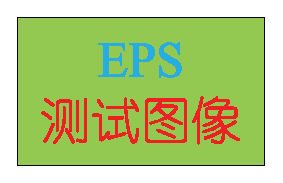
\includegraphics[width=0.3\textwidth]{chap2/testeps}}
  \hspace{1in}
  \subfigure[PDF Figure]{
    \label{fig:epspdf:b} %% label for second subfigure
    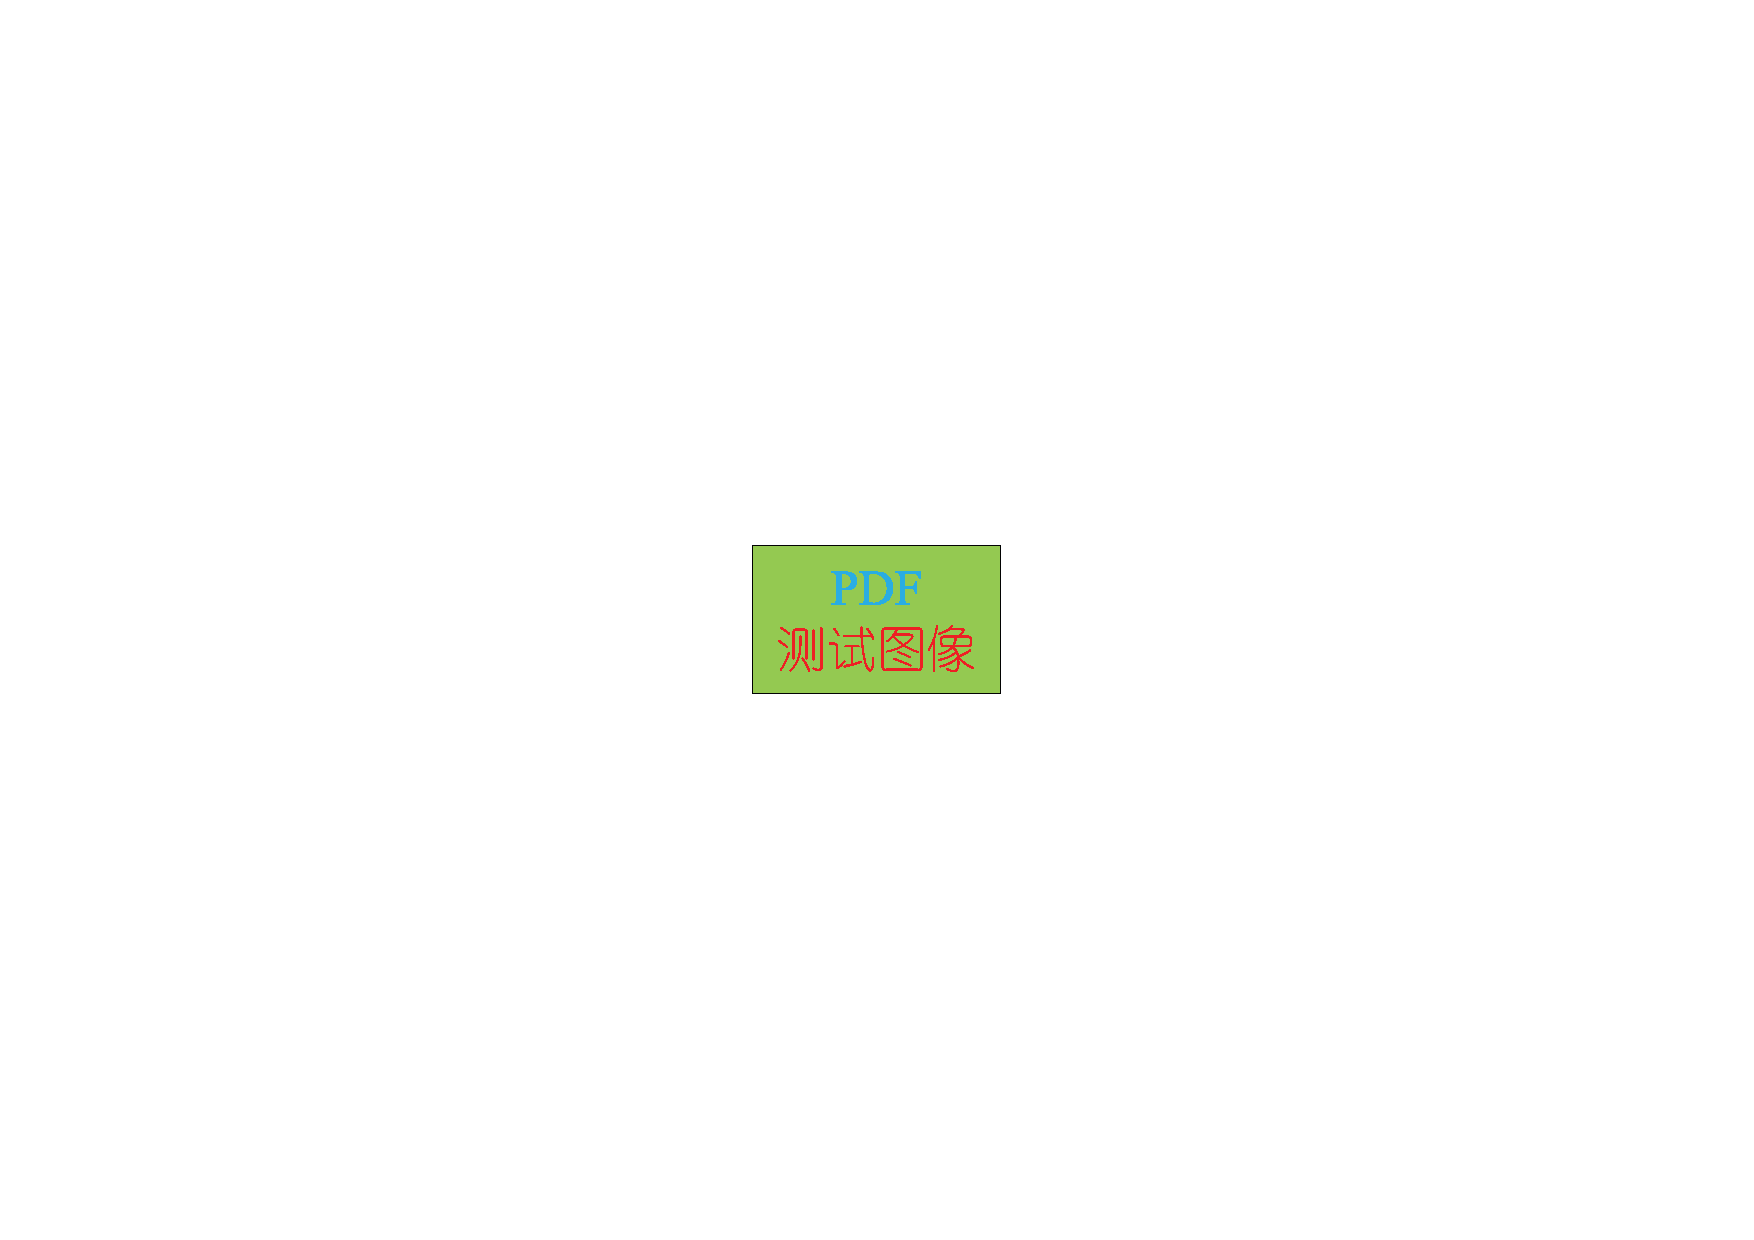
\includegraphics[angle=-90,origin=br,width=0.3\textwidth]{chap2/testpdf.pdf}}
  \bicaption[fig:pdfeps]{插入eps图像和pdf图像}{插入eps和pdf的例子}{Fig}{An EPS and PDF demo}
\end{figure}

更多关于 \LaTeX 插图的例子可以参考\href{http://www.cs.duke.edu/junhu/Graphics3.pdf}{《\LaTeX 插图指南》}。

\subsection{长标题的换行}
\label{sec:longcaption}

图\ref{fig:longcaptionbad}和图\ref{fig:longcaptiongood}都有比较长图标题,通过对比发现,图\ref{fig:longcaptiongood}的换行效果更好一些。
其中使用了minipage环境来限制整个浮动题的宽度。

\begin{figure}[!htp]
 \centering
 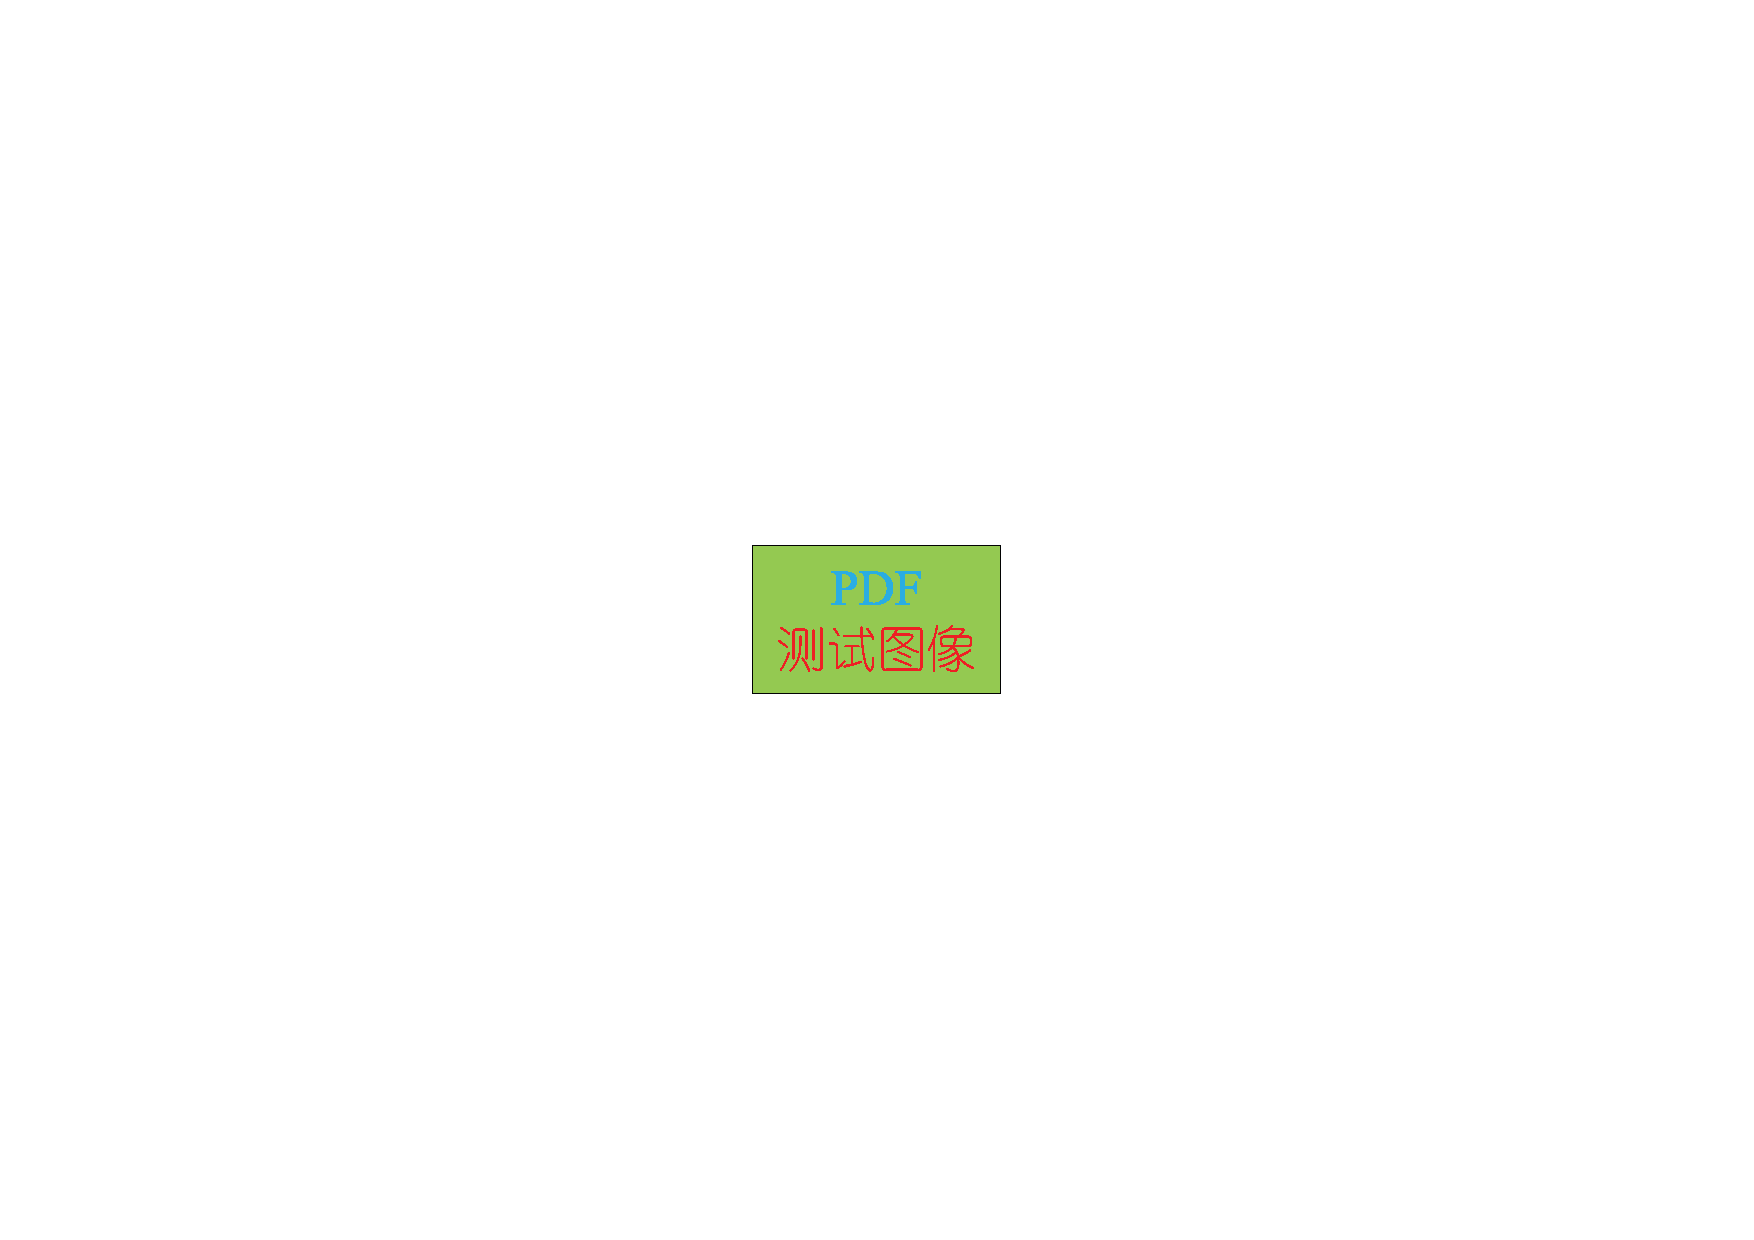
\includegraphics[angle=-90,origin=br,width=4cm]{chap2/testpdf.pdf}
 \bicaption[fig:longcaptionbad]{这里将出现在插图索引}{海交通大学是我国历史最悠久的高等学府之一,是教育部直属、教育部与上海市共建的全国重点大学.}{Fig}{Where there is a will, there is a way.}
\end{figure}


  \begin{figure}[!hbp]
    \centering
    \begin{minipage}[b]{0.6\textwidth}
      \captionstyle{\centering}
      \centering
      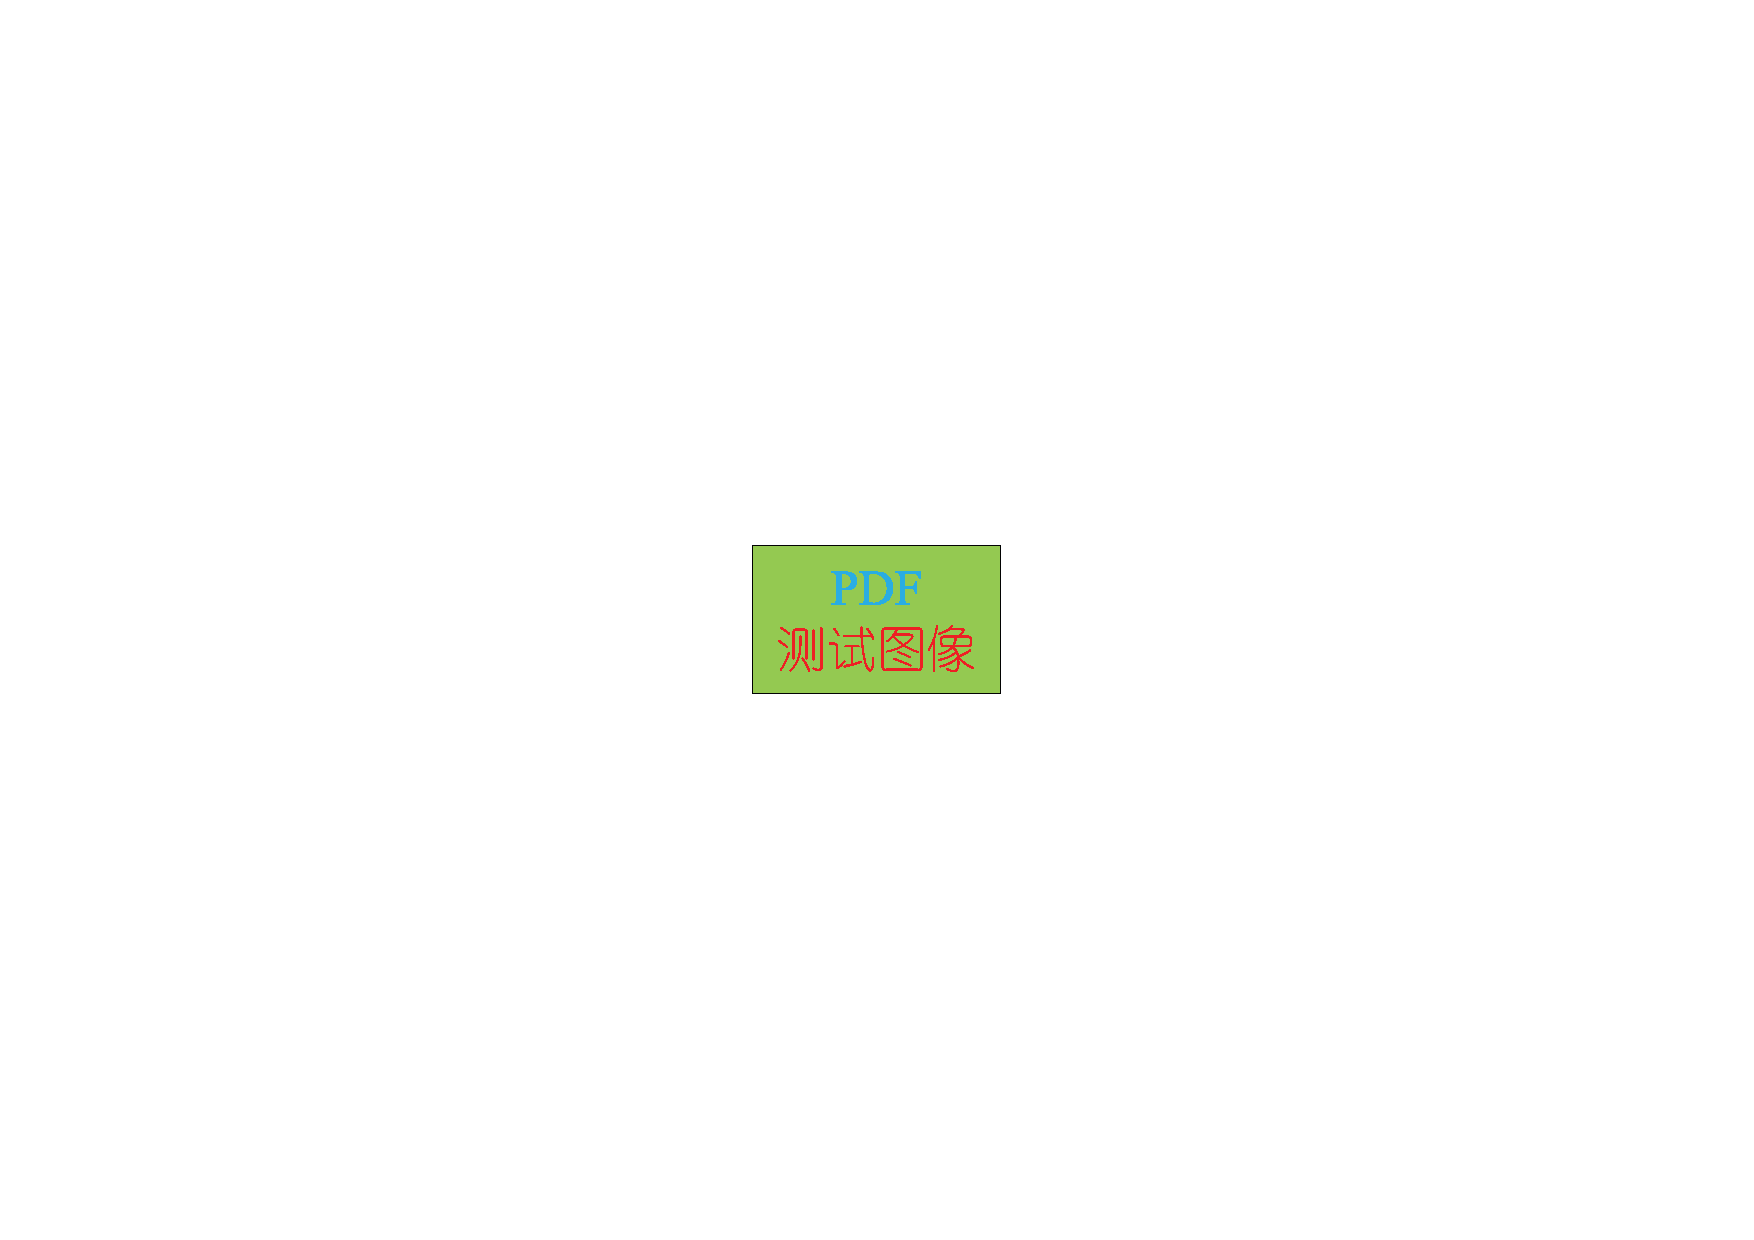
\includegraphics[angle=-90,origin=br,width=4cm]{chap2/testpdf.pdf}
      \bicaption[fig:longcaptiongood]{这里将出现在插图索引}{海交通大学是我国历史最悠久的高等学府之一,是教育部直属、教育部与上海市共建的全国重点大学.}{Fig}{Where there is a will, there is a way.}
    \end{minipage}     
  \end{figure}

  
\section{表格的例子}
\label{sec:tab}

这一节给出的是一些表格的例子,如表\ref{tab:firstone}所示。

\begin{table}[!hpb]
  \centering
  \bicaption[tab:firstone]{指向一个表格的表目录索引}{一个颇为标准的三线表格\footnotemark[1]}{Table}{A Table}
  \begin{tabular}{@{}llr@{}} \toprule
    \multicolumn{2}{c}{Item} \\ \cmidrule(r){1-2}
    Animal & Description & Price (\$)\\ \midrule
    Gnat & per gram & 13.65 \\
    & each & 0.01 \\
    Gnu & stuffed & 92.50 \\
    Emu & stuffed & 33.33 \\
    Armadillo & frozen & 8.99 \\ \bottomrule
  \end{tabular}
\end{table}
\footnotetext[1]{这个例子来自\href{http://www.ctan.org/tex-archive/macros/latex/contrib/booktabs/booktabs.pdf}{《Publication quality tables in LATEX》}(booktabs宏包的文档)。这也是一个在表格中使用脚注的例子,请留意与threeparttable实现的效果有何不同。}

下面一个是一个更复杂的表格,用threeparttable实现带有脚注的表格,如表\ref{tab:footnote}。

\begin{table}[!htpb]
  \bicaption[tab:footnote]{出现在表目录的标题}{一个带有脚注的表格的例子}{Table}{A Table with footnotes}
  \centering
  \begin{threeparttable}[b]
     \begin{tabular}{ccd{4}cccc}
      \toprule
      \multirow{2}{6mm}{total}&\multicolumn{2}{c}{20\tnote{1}} & \multicolumn{2}{c}{40} &  \multicolumn{2}{c}{60}\\
      \cmidrule(lr){2-3}\cmidrule(lr){4-5}\cmidrule(lr){6-7}
      &www & k & www & k & www & k \\
      \midrule
      &$\underset{(2.12)}{4.22}$ & 120.0140\tnote{2} & 333.15 & 0.0411 & 444.99 & 0.1387 \\
      &168.6123 & 10.86 & 255.37 & 0.0353 & 376.14 & 0.1058 \\
      &6.761    & 0.007 & 235.37 & 0.0267 & 348.66 & 0.1010 \\
      \bottomrule
    \end{tabular}
    \begin{tablenotes}
    \item [1] the first note.% or \item [a]
    \item [2] the second note.% or \item [b]
    \end{tablenotes}
  \end{threeparttable}
\end{table}

\section{参考文献管理}

参考文献的管理是这个学位论文模板又一个好玩的地方。

\subsection{将参考文献的内容与表现分离}

这个论文模板使用BibTeX处理参考文献,这又是一个``内容''与``表现形式''分离的极好例子
\footnote{当然,你也可以手动编参考文献item,直接插入文档中。但是,有BibTeX帮助,我觉得没有人想用这种麻烦的方法,所以就在脚注中说明了。}。
参考文献的``内容''就是reference文件夹下的chap\textit{xx}.bib,参考文献的元数据(名称、作者、出处等)以一定的格式保存在这些纯文本文件中。
.bib文件也可以理解为参考文献的``数据库'',正文中所有引用的参考文件条目都会从这些文件中``析出''。
控制参考文献条目``表现形式''(格式)的是.bst文件。.bst文件定义了参考文献风格,使用不同的参考文献风格能将同一个参考文献条目输出成不同的格式。
当然,一个文档只能使用一个参考文献风格。
按照教务处的要求,本模板使用的是国标GBT7714风格的参考文献。

BibTeX的工作过程是这样的:
BibTeX读取.aux(第一次运行latex得到的)看看你引用了什么参考文献条目,
然后到.bib中找相关条目的信息,
最后根据.bst的格式要求将参考文献条目格式化输出,写到.bbl文件中。
在运行latex将.bbl插入文档之前,你可以用文本编辑器打开它,做一些小的修改。
你会发现,.bbl的格式和你自己手动写item很相似,它已经被赋予了一定的``表现形式''。

.bib数据库中的参考文献条目可以手动编写,也可以在google的学术搜索中找到。
各大数据库\footnote{应该说是国际知名数据库,譬如SCOPUS, IEEE, OSA等,国内数据库在搜索、导出方面一直是差得一塌糊涂。}也支持将参考文献信息导出为.bib,
省时省力。
以Google学术搜索为例:进入\url{http://scholar.google.com},在``学术搜索设置''中,将``文献管理软件''设为``显示导入BibTeX''的连接,保存退出。
然后学术搜索找到文献下会有``导出到BibTeX''连接,点击后Firefox会打开新的标签页,出现类似代码\ref{googlescholar}所示的内容
\footnote{展示这些.bib条目使用了listings宏包,因为listings宏包协调中文的能力很糟糕,所以读者在查看模板的这部分源代码时会看到一些非常麻烦的东西。并且,直接将源代码的这部分内容复制到.bib中可能还会出错。我的建议是:这部分内容留意PDF就足够了。}。
请注意,这个条目离``规范''还有一些距离。

  \begin{lstlisting}[caption={从Google Scholar找到的,但并不规范的.bib条目}, label=googlescholar, float, escapeinside="", numbers=none]
    @phdthesis{"白2008信用风险传染模型和信用衍生品的定价",
      title={{"信用风险传染模型和信用衍生品的定价"}},
      author={"白云芬"},
      year={2008},
      school={"上海交通大学"}
    } 
  \end{lstlisting}

  上面的.bib条目的``名字''\cndash{}``白2008信用风险传染模型和信用衍生品的定价'',包含ASCII以外的字符,BibTeX无法处理;
  条目还缺少了address域,这样编译出来的结果会出现``地址不详'';
  并且,条目还缺少language域,BibTeX需要language域来判断是否是中文参考文献。
  将上面的条目修正(改英文名、增加address和language域),复制到本地的.bib文件中就可以了。
  显然,这里描述的是参考文献的内容,而不是表现形式。

  \begin{lstlisting}[caption={一个符合规范的.bib条目}, label=itemok, float, escapeinside="", numbers=none]
    @phdthesis{bai2008,
      title={{"信用风险传染模型和信用衍生品的定价"}},
      author={"白云芬"},
      year={2008},
      language={zh},
      address={"上海"},
      school={"上海交通大学"}
    } 
  \end{lstlisting}

由于中英文参考文献处理起来有差异,所以需要在参考文献中标注是否是中文文献。
确切地说,BibTeX并不具有区分中英文参考文献的``智能'',这种智慧的来源是.bst文——它定义了处理参考文献的规则。
GBT7714-2005NLang.bst中规定:.bib中的条目,如果条目的``language''域非空,就被认为是中文文献,否则被认为是英文文献。
例如,刚才的文献,就会被认为是中文参考文献,采取一些针对中文的处理方式。

最后,这个条目被bibtex处理后,赋予了一定的``表现形式'',在.bbl文件中以下面的样子出现。
你还可以对它进行小的修改,这是一种很折磨人的终极修改方法。
再次运行latex之后,它将被插入到文档中。

\begin{lstlisting}[caption={.bbl中被格式化之后的条目}, escapeinside="", numbers=none]
\bibitem["白云芬(2008)"]{bai2008}
  \textsc{"白云芬"}.
  \newblock {"信用风险传染模型和信用衍生品的定价"}[D].
  \newblock "上海: 上海交通大学, 2008."
\end{lstlisting}

再罗嗦两句,
.bst文件书写起来非常繁杂\footnote{可以参考\href{http://ftp.ctex.org/mirrors/CTAN/info/bibtex/tamethebeast/ttb_en.pdf}{《Tame The BeaST》}。},书写符合GBT7714标准的.bst文件更是一项浩大的工程。
因此,当大家为漂亮、标准的参考文献列表感到满意时,应该对GBT7714-2005NLang.bst的作者充满谢意。
作者在CTeX BBS发的帖子,请看
\href{http://bbs.ctex.org/viewthread.php?tid=33571&highlight=\%B2\%CE\%BF\%BC\%CE\%C4\%CF\%D7\%2BGB}{文后参考文献著录规则 GB/T 7714-2005}。
关于GB/T 7714-2005标准本身,请看\href{http://bbs.ctex.org/viewthread.php?tid=33571&highlight=GB\%2B\%B2\%CE\%BF\%BC\%CE\%C4\%CF\%D7}{这里}。

再多说两句,.bib是“参考文献的内容”,而控制参考文献表现(格式)的是.bst文件,本模板附带的是GBT7714-2005NLang.bst。

\subsection{在正文中引用参考文献}

参考文献可以分章节管理,只需要在主文件中的参考文献中都包含进去就可以,如\verb+\bibliography{chap1,chap2,...}+。

正文中引用参考文献时,用\verb+\upcite{key1,key2,key3...}+可以产生“上标引用的参考文献”,
如\upcite{Meta_CN,chen2007act,DPMG}。
使用\verb+\cite{key1,key2,key3...}+则可以产生水平引用的参考文献,例如\cite{JohnD,zhubajie,IEEE-1363}。
请看下面的例子,将会穿插使用水平的和上标的参考文献:关于书的\cite{Meta_CN,JohnD,IEEE-1363},关于期刊的\upcite{chen2007act,chen2007ewi},
会议论文\cite{DPMG,kocher99,cnproceed},
硕士学位论文\cite{zhubajie,metamori2004},博士学位论文\upcite{shaheshang,FistSystem01,bai2008},标准文件\cite{IEEE-1363},技术报告\upcite{NPB2},电子文献\cite{xiaoyu2001, CHRISTINE1998}。

最后总结一些注意事项:
\begin{itemize}
\item 参考文献只有在正文中被引用了,才会在最后的参考文献列表中出现;
\item 参考文献``数据库文件''.bib是纯文本文件,请使用UTF-8编码,不要使用GBK编码;
\item 参考文献条目中通过language域是否为空判断是否是中文文献;
\item 参考文献条目同样有“内容”和“表现形式”之分,这种可控性是BibTeX带来的。
\end{itemize}


\subsection{参考文献管理器}

参考文献数据库.bib虽然是纯文本的,可以用任意的文本编辑器查看,但总有人喜欢一个找一个``可视化''地查看每一条参考文献。
我想\href{http://jabref.sourceforge.net/}{JabRef}应该是个很不错的选择。
这是一个Java写的程序,需要JRE才能运行。
就我测试的情况上看,很幸运,JabRef可以顺利打开GBK编码的.bib文件。
但是,打开UTF--8编码的.bib源文件过程中总会崩溃,原因不得而知。
由于我们的.bib文件使用的是UTF-8编码,所以JabRef暂时不可用。

提到参考文献管理器,不得不提到另一个广被使用的软件——\href{http://www.endnote.com/}{EndNote}。
在图书馆的宣讲会上,EndNote被吹得神乎其神,但我发现他对.bib的管理很不友好。
EndNote可以导入.bib文件,却不能导出.bib,只能导出.bbl——被格式化的.bib。
原来,JabRef比较``单纯'',不具备格式化参考文献的能力;
而EndNote有那么一点设置参考文献输出格式的能力,然后就把这种能力滥用,这点搞得我很不爽。
看来,EndNote和Word配合得更好一些。


\section{用listings插入源代码}

原先ctexbook文档类和listings宏包配合使用时,代码在换页时会出现莫名其妙的错误,后来经高人指点,顺利解决了。
感兴趣的话,可以看看\href{http://bbs.ctex.org/viewthread.php?tid=53451}{这里}。
这里给使用listings宏包插入源代码的例子,这里是一段C代码。
另外,listings宏包真可谓博大精深,可以实现各种复杂、漂亮的效果,想要进一步学习的同学,可以参考
\href{http://mirror.ctan.org/macros/latex/contrib/listings/listings.pdf}{listings宏包手册}。

\begin{lstlisting}[language={C}, caption={一段C源代码}]
#include <stdio.h>
#include <unistd.h>
#include <sys/types.h>
#include <sys/wait.h>

int main() {
  pid_t pid;

  switch ((pid = fork())) {
  case -1:
    printf("fork failed\n");
    break;
  case 0:
    /* child calls exec */
    execl("/bin/ls", "ls", "-l", (char*)0);
    printf("execl failed\n");
    break;
  default:
    /* parent uses wait to suspend execution until child finishes */
    wait((int*)0);
    printf("is completed\n");
    break;
  }

  return 0;
}
\end{lstlisting}

再给一个插入MATLAB代码的例子,感谢daisying站友提供的代码。

\begin{lstlisting}[language={matlab}, caption={一段MATLAB源代码}]
function paper1
r=0.05;
n=100;
T=1;
X=1;
v0=0.8;
sigma=sqrt(0.08);
deltat=T/n;
for i=1:n
    t(i)=i*deltat;
    w(i)=random('norm',0,t(i),1);
end
for i=1:n
    alpha(i)=0.39;
end
for i=1:n
    temp=0;
    for k=1:i
        temp=temp+alpha(k);
    end
    B(i)=exp(r*t(i));
    BB(i)=B(i)*exp(temp*deltat);
    BBB(i)=exp(-r*(T-t(i)));
end
for i=1:n
    s0(i)=X*BBB(i);
    v(i)=v0*exp((r-0.5*sigma^2)*t(i)+sigma*w(i));
    for j=i+1:n
        D=X*BBB(j);
        d1=(log(v(i)/D)+(r+sigma^2/2)*(t(j)-t(i)))/(sigma*sqrt(t(j)-t(i)));
        d2=d1-(sigma*sqrt(t(j)-t(i)));
        ppp(i,j)=D*exp(-r*(t(j)-t(i)))*(1-cdf('normal',d2,0,1))-v(i)*(1-cdf('n
ormal',d1,0,1));
    end
end
for i=1:n
    s1(i)=0;
    for j=i+1:n
        s1(i)=s1(i)+BB(j)^(-1)*alpha(j)*deltat*(X*BBB(j)-B(j)/B(i)*ppp(i,j));
    end
    s2(i)=0;
    for j=1:n
        s2(i)=s2(i)+alpha(j);
    end
    s2(i)=X*exp(-r*T-s2(i)*deltat);
    s(i)=BB(i)*(s1(i)+s2(i));
end
plot(s)
hold on;
plot(s0);
\end{lstlisting}

%%%==================================================
%% chapter03.tex for SJTU Master Thesis
%% Encoding: UTF-8
%%==================================================

\chapter{常见问题与故障排除}
\label{chap:faq}

\subsubsection*{我是否能够自由使用这份模板}
是的,你可以自由使用这份模板。但将模板用于商业用于以前,请征得我的同意。

\subsubsection*{我的论文是Word排版的,学校图书馆是不是只收 \LaTeX 排版的论文}
当然不是,Word版肯定收。

\subsubsection*{我的论文是 \LaTeX 排版的,学校图书馆是不是只收Word排版的论文}
当然不是,PDF版的电子论文是可以上交的。是否要交Word版就看你导师的喜好了。

\subsubsection*{为什么左右页边距不一样}
模板默认是双面打印,迎面页和背面页的页边距是要交换的,多出来的那一部分是留作装订的。

\subsubsection*{为什么在参考文献中会有``//''符号}
那就是国标GBT7714参考文献风格规定的。

\subsubsection*{为什么参考文献中会有[s.n.],[S.l], [EB/OL]等符号}
那也是国标GBT7714参考文献风格定义的。[s.n.]表示出版者不祥,[S.l]表示出版地不祥,[EB/OL]表示引用的参考文献类型为在线电子文档。

\subsubsection*{如何获得帮助和反馈意见}
你可以通过如下的途径反馈模板使用过程中遇到的问题:\href{https://github.com/weijianwen/sjtu-thesis-template-latex/issues}{开issue}
、\href{https://bbs.sjtu.edu.cn/bbsdoc?board=TeX_LaTeX}{水源LaTeX版}发帖,或者是给\href{mailto:weijianwen@gmail.com}{我}发送邮件---你可能需要好几天才能收到我的邮件回复。

\subsubsection*{使用文本编辑器查看tex文件时遇到乱码}
请确保你的文本编辑器使用UTF-8编码打开了tex源文件。

\subsubsection*{在CTeX编译模板遇到``rsfs10.tfm already exists''的错误提示}
请删除\verb+X:\CTEX\UserData\fonts\tfm\public\rsfs+下的文件再重新编译。问题讨论见\href{https://bbs.sjtu.edu.cn/bbstcon,board,TeX_LaTeX,reid,1352982719.html}{水源2023号帖}。

\subsubsection*{升级了TeXLive 2012,编译后的文档出现``minus''等字样}
这是xltxtra和fontspec宏包导致的问题。学位论文模板从0.5起使用metatlog宏包代替xltxtra生成 \XeTeX 标志,解决了这个问题。

\subsubsection*{如何向你表示感谢}
请在项目的\href{https://github.com/weijianwen/sjtu-thesis-template-latex}{github主页}点击``Star'',我想粗略统计一下使用学位论文模板的人数,谢谢。

\chapter{距离度量学习}
\label{chap:dca}

在本章中,我们解决如何利用已知的局部信息网络的信息去学习一个距离度量,
并通过这个度量计算任意节点对之间的距离。

欧式距离是一种简单的计算节点之间距离的方法,
它仅仅利用两个节点的属性向量去计算两个节点之间的距离。
有时,节点之间的距离不仅仅和节点的属性有关,
因此需要一种方法在欧式距离的基础上进行一定的调整,
让已知的相似的节点之间的距离更近一些,而让不相似的节点之间的距离更远一些。
在这种情况下,我们采用马氏距离来表示节点之间的距离,
而计算马式距离的最主要的任务是要求得马氏转换矩阵(Mahalanobis matrix)$M$。

\section{问题的数学定义}
\label{sec:dcadef}

\begin{defn}{正语境限制}
\label{defn:posconstraints}

    正语境限制是指已知某些节点之间是相似的。
    正语境限制通过一个相似集列表$C$给出,
    $C$中的每一个元素$C_i$都代表一个由相似的节点组成的集合。
    即:

    $$
    x_i\text{与}x_j\text{相似} \Longleftrightarrow \exists k \ x_i \in C_k \text{且} x_j \in C_k 
    $$

\end{defn}

\begin{defn}{负语境限制}
\label{defn:negconstraints}

    负语境限制限定了正语境中规定的相似集之间是否是不相似的。
    负语境限制通过一个与$C$同样长度的列表$D$给出,
    对于每一个$C_i$,$D_i$表示$C$中所有与$C_i$不相似的相似集组成的结合。
    即:

    $$
    D_i = \{C_j | C_i \text{与} C_j \text{不相似} \}
    $$

\end{defn}

利用局部信息网络,我们可以得到正语境限制和负语境限制。
已知数据集
$X = \{ \bm{x}_i \}_{i=1}^{N}$
以及在数据集上的正语境限制$C$和负语境限制$D$,
$C$和$D$的长度都为$n$,
判别成分分析(Discriminative Component Analysis,DCA)算法
通过学习一个转换矩阵$M$,使得通过这个矩阵计算出的节点距离让相似的节点之间的距离更近,
不相似的的节点之间的距离更远。

为了完成判别成分分析,定义两个协方差矩阵$\hat{C_b}$和$\hat{C_w}$分别表示
相似集之间的总方差和相似集内部的总方差。$\hat{C_b}$和$\hat{C_w}$的定义如下:

\begin{align}
    \hat{C_b} &= \frac{1}{n_b} \sum_{j=1}^n \sum_{i \in D_j} (\bm{m}_j - \bm{m}_i)(\bm{m}_j - \bm{m}_i)^\top \\
    \hat{C_w} &= \frac{1}{n_b} \sum_{j=1}^n \frac{1}{n_j} \sum_{i = 1}^{n_j} (\bm{x}_{ij} - \bm{m}_j)(\bm{x}_{ij} - \bm{m}_j)^\top
\end{align}

其中$n_b = \sum_{j=1}^{n}|D_j|$, $|\bullet|$表示集合的基数,
$n_j = |C_j|$,
$\bm{m}_j$表示相似集$C_j$的平均向量,亦即
$\bm{m}_j = \frac{1}{n_j} \sum_{i=1}^{n_j} \bm{x}_{ji}$, 
$\bm{x}_{ji}$是指$C_j$中的第$i$个元素。

DCA算法的目的是找到一个对于距离度量的最优线性转换
使得相似集之间的总方差最大而相似集内部的总方差最小,
也就是求解下面的最优化问题:

\begin{equation}
    \label{equa:dca_opt}
    J(A) = \operatorname*{arg\,max}_A \frac {|A^\top \hat{C_b} A|} {|A^\top \hat{C_w} A|}
\end{equation}

当找到最优的$A$, 最优的马氏转换矩阵也就是$M = A^\top A$。

\section{DCA算法的求解}
\label{sec:algorithm_dca}

根据Fisher定理\upcite{mika1999fisher},
等式\ref{equa:dca_opt}的最优解是一个同时使$\hat{C_b}$和$\hat{C_w}$对角化的转换矩阵。
求解的详细过程如下:

\begin{itemize}
    \item 使用特征分析把$\hat{C_b}$对角化: 
        \begin{itemize}
            \item 找到一个矩阵$U$满足$U^\top \hat{C_b} U = \Lambda_b, U^\top U = I$,
                其中$\Lambda_b$是一个升序的对角矩阵;
            \item 选取$U$的后面$k$个特征值不为$0$的特征向量组成矩阵$\hat{U}$;
            \item 求得$D_b = \hat{U}^\top\hat{C_b}\hat{U}$;
            \item 求得$Z = \hat{U}D_b^{-1/2}, C_z = Z^\top\hat{C_w}Z$;
        \end{itemize}

    \item 使用特征分析把$C_z$对角化: 

        找到一个矩阵$V$满足$V^\top C_z V = \Lambda_w, V^\top V = I$,
                其中$\Lambda_w$是一个升序的对角矩阵。

    \item 最终$A = Z\hat{V}\Lambda_w^{-1/2}, M = A^\top A$。 
        
\end{itemize}

DCA算法具体实现见\ref{code:dca}


\section{本章小节}

在本章中,我们提出了一种距离度量学习的算法——DCA,
它能够利用信息网络的节点属性$X$,正语境限制$C$和负语境限制$D$,
使用DCA算法学习距离度量矩阵$M$,
通过$M$计算出的节点对之间的距离能够保证相似的节点之间拥有更近的距离。

\chapter{基于距离的聚类算法--DSHRINK}
\label{chap:dshrink}

在第\ref{chap:dca}章中,我们获得了一个距离学习度量,
利用它,可以计算任意两个节点$u, v$之间的距离$d(u, v)$。
本章介绍一种基于距离进行层次化聚类方法DSHRINK,
它通过不断地把一些节点组合到一起形成一个超级节点,
直到碰到终止条件停止聚类。

\section{基于距离的模块性准测}

DSHRINK算法总是试图把相邻的节点聚到一起组成一个超级节点,
然后超级节点又会跟其他的节点进行聚类,如果没有终止条件,
那最后所有的节点会被聚到一类。模块性准测是一种评价聚类质量的方法,
如果把一些节点聚到一起,会造成聚类质量不好,就停止聚类。

\begin{defn}{基于距离的模块性}
    \label{defn:density-based-modularity}

    给定不完全信息网络$G = (V, E, A, M)$和在它上面的聚类
    $C = \{C_1, C_2, ..., C_k\}$, 基于距离的模块性$Q_d$为:

    \begin{equation}
    Q_d = \sum_{i=1}^k [ \frac{D_i^I}{D^T} - (\frac{D_i^C}{D^T})^2]
    \end{equation}

    其中$k$是聚类的数目,
    $D_i^I = \sum_{u,v \in C_i} d(u,v)$是聚类$C_i$中任意两节点的距离和,
    $D_i^C = \sum_{u \in C_i, v \in V} d(u,v)$是聚类$C_i$中任意一个节点和其他节点的距离和,
    $D^T = \sum_{u,v \in V} d(u,v)$是任意两节点的距离和。

\end{defn}

显然,模块性的取值范围是$[-1,0]$,如果$Q_d = 0$,那么要么所有节点都在同一个聚类,
要么所有节点都在不同的聚类。$Q_d$越小,聚类的质量越好。

如果我们把任意的两个聚类$C_s$和$C_t$合并成了一个聚类,
那么模块性的增量$\Delta Q_d$为:

\begin{equation}
\label{equa:delta-qd}
    \Delta Q_d = Q_d^{C_s \bigcup C_t} - Q_d^{C_s} - Q_d^{C_t} = \frac{2D_{st}^U}{D^T} - \frac{2D_s^CD_t^C}{(D^T)^2}
\end{equation}

其中$D_{st}^U = \sum_{u \in C_s, v \in C_t} d(u,v)$是聚类$C_s$中任意节点与聚类$C_t$中任意节点的距离和。

根据等式\ref{equa:delta-qd}, 当把$j$个聚类$C_1, C_2, ..., C_j$合并成一个聚类时,
模块性增量$\Delta Q_d$为:

\begin{equation}
\label{equa:delta-qd2}
\Delta Q_d = \frac{\sum_{s,t \in {1,...,j}, s \neq t }2D_{st}^U}{D^T} - \frac{\sum_{s,t \in {1,...,j}, s \neq t }2D_s^CD_t^C}{(D^T)^2}
\end{equation}

\section{DSHRINK聚类算法}

在详细讲述DSHRINK算法之前,先给出一组定义。

\begin{defn}{最近邻居}
    \label{defn:nearest-neighbor}

    给定一个不完全信息网络$G = (V, E, A, M)$,
    任意节点$u$的最近邻居集是:

    \begin{equation}
        NN(v) = \{y | y = \operatorname*{arg\,min}_x d(u, x), x \in V \wedge x \neq v\}
    \end{equation}

\end{defn}

\begin{defn}{互近邻}
    \label{defn:mnn}

    给定一个不完全信息网络$G = (V, E, A, M)$,
    节点$u, v$被称为互近邻,标记为:
    $ u \xleftrightarrow{\gamma} v, iff v \in NN(u) \wedge u \in NN(v) \wedge d(u, v) = \gamma$。

\end{defn}

\begin{defn}{当地社区}

    给定一个不完全信息网络$G = (V, E, A, M)$,
    我们把它的子图$C(v) = (V^\prime, E^\prime, A^\prime, M, \gamma)$叫作一个当地社区如果$
    (1) v \in V^\prime;
    (2) \forall u \in V^\prime, \exists v \in V^\prime \wedge u \xleftrightarrow{\gamma} v;
    (3) \{u | u \in V^\prime \wedge u \xleftrightarrow{\gamma} v \wedge v \notin V^\prime \} = \emptyset
    $。
    
\end{defn}

DSHRINK就是通过不断地把当地社区中的节点组合成一个超级节点,直到终止条件成立来完成整个聚类的过程。
由于当地社区的社区十分严格,要求其中所有的节点都互为最近邻,每一轮迭代组合的节点太少,
会导致整个聚类算法运行时间很长。因此,接下来给出一种更加松弛的当地社区定义。

\begin{defn}{$\epsilon$近似互近邻}
    给定一个不完全信息网络$G = (V, E, A, M)$,
    节点$u, v$被称为$\epsilon$近似互近邻,标记为:
    $ u \xleftrightarrow[\epsilon]{} v, iff 
    (v \in NN(u) \wedge |d(u, v) - d(v, x)| \leq \epsilon) \vee
    (u \in NN(v) \wedge |d(u, v) - d(u, y)| \leq \epsilon)
    $。其中$
    x \in NN(v), y \in NN(u), \epsilon \in R^+
    $
\end{defn}

显然,近似互近邻是对于互近邻的一种扩展,如果两个节点是互近邻,
那么它们一定是近似互近邻,反之则不成立。

\begin{defn}{$\epsilon$近似当地社区}
    \label{defn:local-community}

    给定一个不完全信息网络$G = (V, E, A, M)$,
    我们把它的子图$C(v) = (V^\prime, E^\prime, A^\prime, M, \epsilon)$叫作一个$\epsilon$近似当地社区如果$
    (1) v \in V^\prime;
    (2) \forall u \in V^\prime, \exists v \in V^\prime \wedge u \xleftrightarrow[\epsilon]{} v;
    (3) \{u | u \in V^\prime \wedge u \xleftrightarrow[\epsilon]{} v \wedge v \notin V^\prime \} = \emptyset
    (4) \text{如果} f(r) = \{r | r = d(s, t), s \xleftrightarrow[\epsilon]{} t \wedge s \in V^\prime \wedge t \in V^\prime \}, |max(f(r)) = min(f(r))| \leq \epsilon
    $
    (5) 如果(3)和(4)不能同时被满足,要先保证(4)被满足。

    要满足条件(3)需要往当地社区中添加更多的节点,但是添加节点之后就会使得任意两个节点距离的最大值变大,
    任意两个节点距离的最小值变小,可能会导致条件(4)不满足,根据条件(5),此时因该停止添加。

\end{defn}

采用近似当地社区取代当地社区用于组合生成超级节点能够极大地加快整个聚类的过程。
原来两个不是互近邻的节点有可能就是$\epsilon$近似互近邻,因此,
每一次能够把更多的节点聚到一起,使每一次迭代的步调能够更大。
而且,通过我们实验观察得知,最终的聚类效果几乎与$\epsilon$的取值无关。
因此,选定一个合适的$\epsilon$,就能极大地减少整个算法所需要的时间,
而且不会影响最终结果的质量。

DSHRINK算法的详细过程如算法\ref{algo:dshrink}所示。
整个算法分为两个部分,前面的初始化部分和后面聚类部分。
在初始化时,除了初始化每一个节点成一个单独的聚类,还有一个重要的步骤就是计算$S_i^T$和$D^T$。
对于任何一个节点$v_i$,所有节点和它的距离和是$s_i^T$,而任意两个节点对的距离和是$D^T$。
在等式\ref{equa:delta-qd2}计算$\Delta Q_d$时需要$D^T$,
而$D_s^C = \sum_{v_i \in C_s, v_j \in V} d(v_i, v_j) = \sum_{v_i \in C_s} S_i^T$,
所以提前计算出$S_i^T$和$D_i^T$能够节省一定的计算量。

算法的第二部分就是不断地迭代,每次迭代把当地社区组合成一个超级节点,
直到组合所有找到的当地社区都会导致$\Delta Q_d \geq 0$,循环终止,
此时聚类结束。每一个超级节点就是一个社区。关于算法的实现细节,有几点需要补充说明:

\begin{itemize}
    \item 在每次循环时,需要找到一个当地社区列表,我们挑选C中的任何一个超级节点作为起始节点,
    然后使用BFS添加节点到当前的社区。此时需要注意不要违反定义\ref{defn:local-community}中的条件(4)。
    当遍历到一个节点时,可以把它的$\epsilon$近似互近邻按照和当前节点的距离进行排序,
    距离更近的节点更先被访问。当然,也可以把这个排序的步骤放在算法\ref{algo:dshrink}的第22行完成。

    \item 在每次把一个当地社区组合成一个超级节点之后,需要重新计算这个超级节点和其他节点之间的距离,
    如果这个距离设置得太小,会造成一个滚雪球效应,拥有节点个数多的聚类与其他节点的距离将会更近,
    这样会更容易和其他的节点聚为一类,从而有导致新生成的聚类拥有更多的节点。因此,
    在计算超级节点与其他节点距离的时候,不能简单地选取聚类中所有节点与超级节点的最小值作为距离,
    需要根据数据的特点确定使用最小值还是平均值,甚至是最大值。
\end{itemize}


\begin{algorithm}[htb]
    \caption{DSHRINK算法}
    \label{algo:dshrink}
    \begin{algorithmic}[1]
        \Require
        不完全信息网络$G = (V, E, A, M)$
        \Ensure
        聚类的集合$C = \{C_1, C_2, ..., C_k\}$
        \State 根据距离度量计算节点之间的距离;
        \State 初始化:把所有的节点作为一个单独的聚类,同时计算每一个节点的$\epsilon$近似互近邻,
        $S^T = 0, D^T = 0, C = \{\{v\} | v \in V \}$;

        \For{each $v_i \in V$}
            \For {each $v_j \in V$}
                \State $S_i^T += d(v_i, v_j)$;
                \State $D^T += d(v_i, v_j)$;
            \EndFor
        \EndFor

        \While {true}
            \State 根据定义\ref{defn:local-community}找到一个当地社区列表$community-list$;
            \State $Q_d.decrease = false$;

            \For {each $community \in community-list$}
                \State 根据等式\ref{equa:delta-qd2}计算$\Delta Q_d$;
                \If {$\Delta Q_d < 0$}
                    \State $Q_d.decrease = true$;
                    \State 把$community$中的聚类组合成一个新的聚类,把$community$中的聚类从$C$中移除,
                    并把这个新添加的聚类加入$C$中;
                \EndIf
            \EndFor

            \If {$!(Q_d.decrease)$}
                \State $break$;
            \EndIf

            \State 重新计算$C$中的超级节点之间的距离,并计算它们的$\epsilon$近似互近邻。
        \EndWhile

        \Return C;

    \end{algorithmic}
\end{algorithm}

DSHRINK的实现代码见\ref{code:dshrink}。

\section{对于DSHRINK算法的分析}

从当地社区或$\epsilon$近似当地社区的定义可知,
节点的访问顺序对于最终寻找的当地社区列表是没有什么影响的。
而且,从整个过程来看,距离更近的节点会更早地被聚在一起,形成一个超级节点。

\section{本章小节}

在本章中,我们详细阐述了使用基于距离的聚类算法DSHRINK用于社区挖掘。
DSHRINK通过不断地把距离较近的节点聚到一起形成一个超级节点来完成聚类的过程。
使用模块性准则作为聚类终止的判断条件。通过实际的实验可知,
采用$\epsilon$近似的DSHRINK聚类算法极大的减少了聚类的运行时间,加快了聚类的速度。

\chapter{实验步骤与实验结果}
\label{chap:implementation}

在这个部分中,我们讲述算法实现的具体步骤以及实验结果。
利用两组数据集,先生成满足条件的不完整信息网络,
然后使用距离学习算法学习距离。通过对比本文算法与kmeans算法的结果,
验证本文算法的可用性。

\section{实验环境}

CPU:Intel(R) Xeor(R) CPU E7420 @ 2.13GHz

内存:64G

操作系统:Microsoft Windows Server 2003 Enterprise x64 Edition

其中采用Python语言实现DSHRINK算法和局部信息网络的生成以及一些自动处理的脚本,
Python的版本是Python2.7。使用Matlab完成DCA算法,PCA分析以及画出结果图,
MATLAB版本为MATLAB version 7.8.0(R2009 a) 64位版 。

\section{社区挖掘的流程}

本文算法的整个流程如图\ref{fig:flow_chart}:

\begin{itemize}
    \item 首先选取合适的数据集用于实验;
    \item 由于数据集所得到的信息网络是完整的,需要对信息网络进行处理,使之满足满足本文关于局部信息网络的定义,
        也就是生成一个信息网络$G$,知道每一个节点的属性$X$,以及正语境限制$C$和负语境限制$D$;
    \item 基于$X, C, D$使用DCA学习一个距离度量,并计算节点对之间的距离;
    \item 基于距离用DSHRINK进行聚类。
\end{itemize}

\begin{figure}
    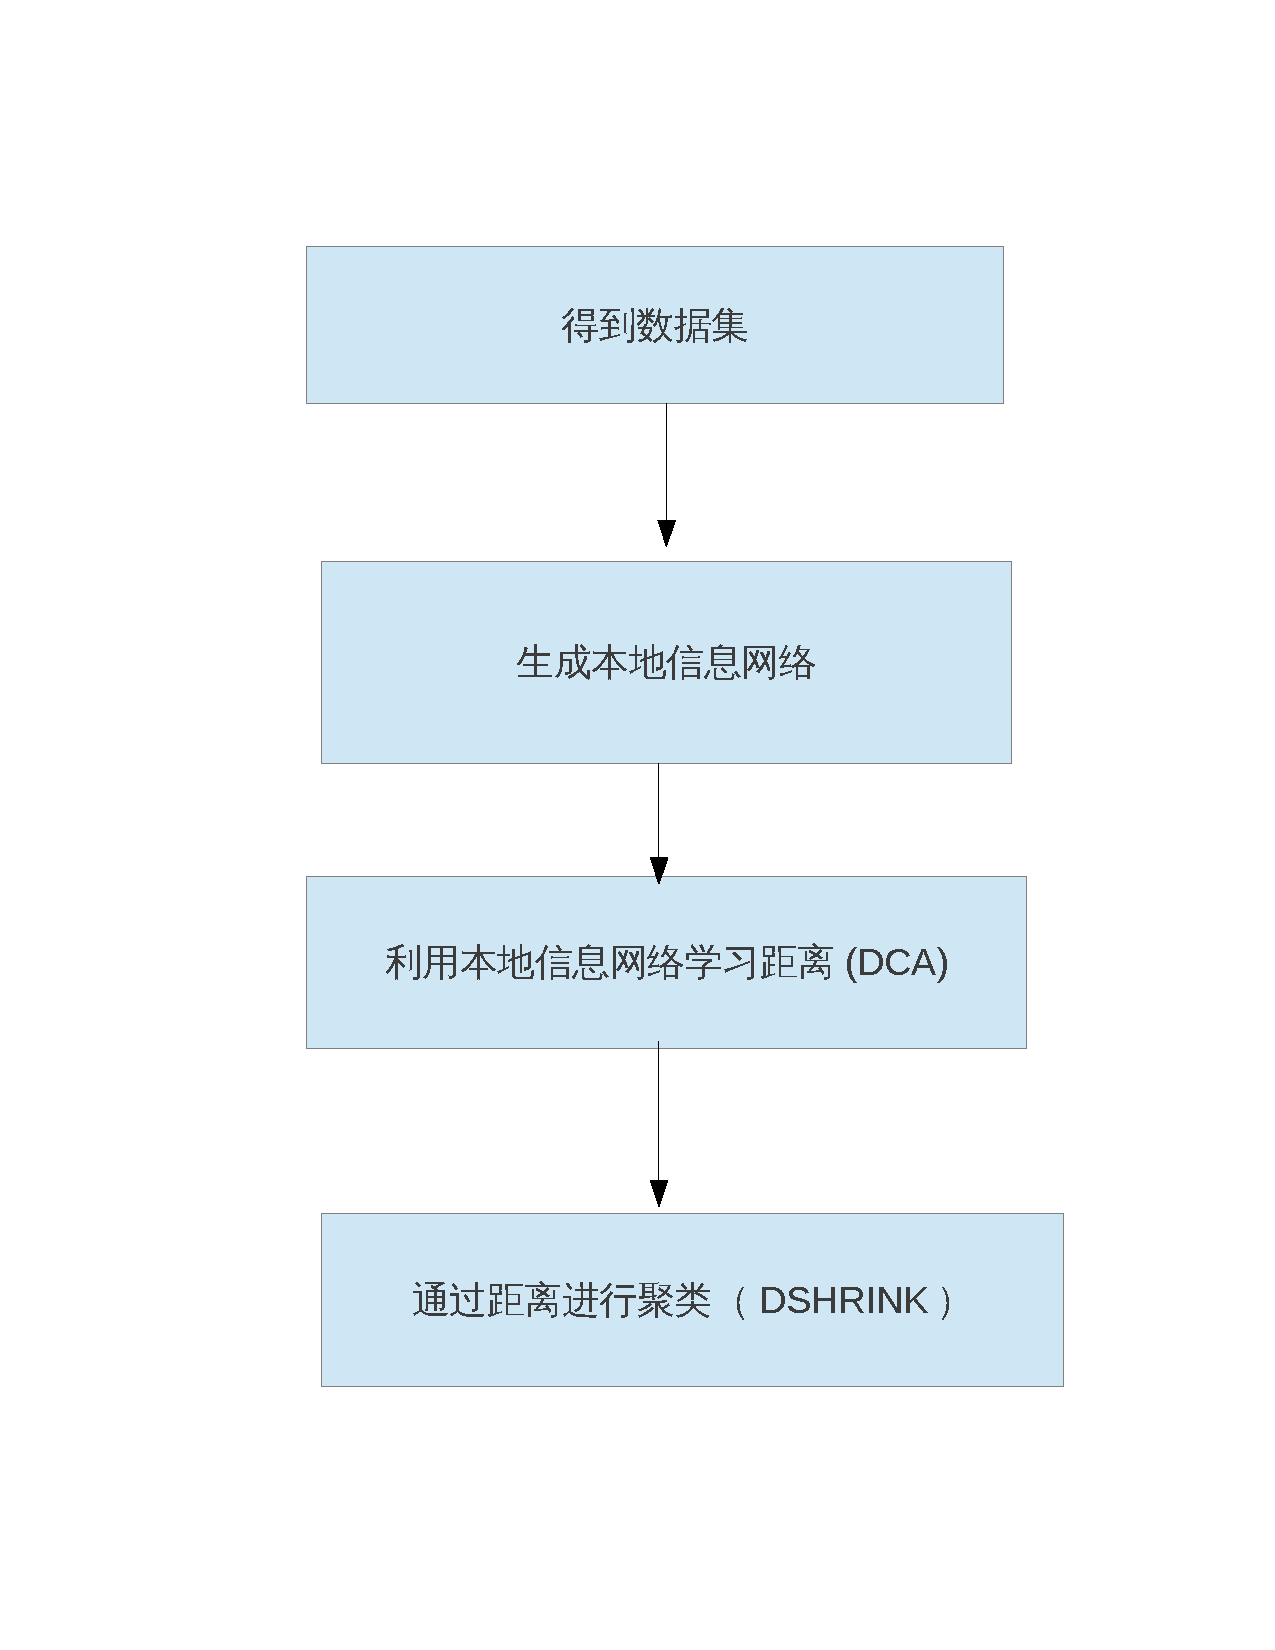
\includegraphics[width=1\textwidth]{flow_chart}
    \caption{社区挖掘的流程}
    \label{fig:flow_chart}
\end{figure}

在本章接下来的几节中,将对每个步骤做具体的介绍。

\section{数据集的选取}
\label{sec:imple:dataset}

本文实验使用两组数据集,均来自于
\href{http://www.blogcatalog.com/}{Blogcatalog},
Blogcatalog是一个博客社交网络, 它把人们与博客作者及博客作者与博客作者联系起来,
从Blogcatalog的数据中,我们可以得到由用户组成的社交网络。
经过处理,我们得到了一个由88784个节点组成的社交网络,每一个节点拥有5413个特征属性。
有60个类作为Ground Truth验证最后的聚类结果,其中每个节点属于60个类中的一个或多个。

由于节点数目过多,所以通过取样的方式生成两组数据集,对于每一组数据集取样的方法如下:
首先从60个中选取6个包含1000个左右节点的类,然后选取属于这6个类中的所有节点作为当前的数据集中的节点。
通过这种方式,得到了数据集Blogcatalog-a和Blogcatalog-b,分别包含5118和5209个节点。

在选定了节点之后,需要对节点的属性进行处理,因为对于每一个节点,大部分属性值都是0,
这样的属性不适合用欧氏距离或马氏距离作为节点之间的距离。所以采用主成分分析(Principle Component Analysis,PCA)对节点的属性进行降唯,
最终选定了50个属性作为节点的属性。在使用PCA分析之前,必须对节点的属性正规化(Normalize)。

最终数据集的特征总结见表\ref{tab:datasetsummary}。

\begin{table}[!hpb]
  \centering
  \caption{实验采用数据集总结}
  \label{tab:datasetsummary}
  \begin{tabular}{rrrrr} \toprule
    数据集 & 节点数 & 边数  & 属性数 & 类个数\\ \midrule
    Blogcatalog-a & 5118 & 22863 & 50 & 6 \\
    Blogcatalog-b & 5118 & 25761  & 50 & 6 \\ \bottomrule
  \end{tabular}
\end{table}


\section{生成局部信息网络}

为了使用DCA距离学习算法,必须生成满足条件的不完全信息网络。
也就是说,必须要生成正语境限制和负语境限制。
本文生成正语境限制和负语境限制的方法如下:

为了生成正语境限制,必须找到相似集列表$C$,
需要在整个信息网络中取样一定数目的节点来生成$C$,
利用局部信息网络的特点,可以通过生成一定数量的特定大小的局部信息网络,
利用这些局部信息网络中的节点来生成$C$。定义局部信息网络的个数为regionNum,
局部信息网络的大小为regionSize。我们首先对节点按照与节点想关联的边的个数进行排序,
然后依次挑选一个节点作为一个局部信息网络的起始节点。对于第一个局部信息网络,
拥有边最多的节点被选中作为其实节点,然后利用宽度优先搜索(Broad First Search, BFS)添加节点到当前的局部信息网络,
直到regionSize个节点被添加。同样地,从排序的节点的列表中挑选边最多的未被访问的节点作为第二个局部信息网络的起始节点,
然后使用BFS添加节点,
依次类推直到生成regionNum个局部信息网络。利用这regionNum个局部信息网络所包含的节点来生成正语境限制。
对于任意两个节点,如果它们属于同样的类,那么它们就是相似的节点对,应该属于同样的相似集。
如果相似集$C_i$中的某个节点与相似集$C_j$相似,那么把$C_i$和$C_j$合并成一个相似集。

生成负语境限制的方法相对简单,只需要随机选取regionNum乘regionSize个节点用于生成负语境限制。
如果相似集$C_i$中的某个节点与相似集$C_j$不相似,那么$j \in D_i$且$i \in D_j$。

在已知了相似节点对列表S和不相似节点对列表D之后,生成正负语境限制的详细过程见\ref{code:constraint},
S的格式$[(u_1, v_1), (u_2, v_2), ...]$其中每一项对应的两个节点都相似,
D的格式$[(u_1, v_1), (u_2, v_2), ...]$其中每一项对应的两个节点都不相似,
输出chunks, 正语境限制和neglinks, 负语境限制。
首先初始化chunks, 每一个节点都没有分配chunk,对应的chunkId是-1。
然后遍历S,生成正语境限制。对于S中任意节点对u,v:
\begin{inparaenum}[a)]
    \item 如果它们都没有分配chunk, 把他们分配到一个新的chunk里;
    \item 如果只是其中一个没有分配chunk,把它分配到另一个的chunk;
    \item 如果两个都分配了chunk,那么合并这两个chunk。
\end{inparaenum}
然后开始生成负语境限制,首先初始化为neglinks为全0矩阵,
也就是说对于任意两个chunks来说,它们不相似的程度为0。
然后遍历D更新neglinks,对于D中的任意两个节点u,v,
如果他们属于不同的已经分配的chunks,那么对应的neglinks加1。

\section{结果好坏的评价标准}

为了评价本文提出算法的有效性,通过对比本文提出的算法和kmeans在Blogcatalog和
Blogcatalog-b上结果的好坏来判定。基于Ground Truth中包含的类的信息,我们使用聚类的纯度(Purity)来作为结果好坏的标准。
纯度的定义如下:

对于每一个聚类,在这个聚类中拥有最多节点个数的类作为这个聚类的标签,
属于这个标签的节点的个数是聚类的标签计数,
纯度等于所有聚类的标签计数和除以所有的节点个数。
数学表达为:

\begin{equation}
\label{equa:purity}
Purity = \frac{1}{n} \sum_{i=1}^k \operatorname{max}_j |C_i \bigcap l_j|
\end{equation}

其中$\{C_1, ..., C_k\}$是所有的聚类,$\{l_1, ..., l_j\}$是所有的类。
根据定义可以知道,纯度越高,聚类的效果越好。

计算纯度的代码见\ref{code:purity}。

\begin{lstlisting}[language={python}, caption={计算聚类的纯度}, label=code:purity]

# 根据划分的聚类计算纯度
# 输入clusters: 得到的一个个聚类
# 输入NODE_NUM: 节点的个数
# 输入usercategory: 用于验证
def get_purity(clusters, NODE_NUM, usercategory):
    purity_sum = 0 # 所有类的标签计数的和,初始化为0

    for cluster in clusters:
        purity_sum += get_max_pi(cluster, usercategory)

    return float(purity_sum) / NUM_NODES #返回标签计数的和除以节点个数作为纯度

# 得到一个聚类的标签计数
# 输入cluster: 聚类,节点列表[c_1, c_2...] 
# 输入usercategory: 用于验证
def get_max_pi(cluster, usercategory):
    category_count = [0] * NUM_CATEGORY #需要统计每一个类所拥有的节点个数,初始化都为0
    
    # 如果有一个节点属于某一个类,那么这个类的节点个数加1
    for node in cluster:
        for category in range(NUM_CATEGORY):
            if usercategory[node][category] == '1':
                category_count[category] += 1

    return max(category_count) #返回所有类中最大的节点个数作为这个聚类的标签计数

\end{lstlisting}


\section{自动化实验}

在完成本文实验的过程中,需要观察DSHRINK和Kmeans在两组数据集下的结果。
对于每一个数据集,需要考察在不同的局部信息网络大小和不同的局部信息网络个数下的纯度,
而且,对于每一种情况都需要重复实验5次去平均值作为实验结果。
这需要进行大量的实验,因此需要一种自动化完成实验的方法。
为此,我们实现了一个自动化的脚本,
运行一次这个脚本能够完成整个实验的过程。

自动化脚本的实现代码见\ref{code:auto}, 分别两组数据集Blogcatalog-a和Blogcatalog-b进行实验,对于每个数据集,
分别研究在不同的局部信息网络大小和不同的局部信息网络个数下面社区挖掘的结果,同时对于每一种情况,重复实验5次,
取平均值作为实验结果。在每次实验时,首先生成正负语境限制,然后利用DCA算法进行距离度量学习,
然后调用DSHRINK算法进行聚类,最后计算出聚类的纯度。

\section{实验结果}
\label{sec:results}
对于数据集Blogcatalog-a和Blogcatalog-b,
分别观察在不同的局部信息网络大小(一个局部信息网络中的节点个数)
和不同的局部信息网络的个数情况下的实验结果。
由于算法具有一定的随机性,对于每一种不同的情况,
重复实验5次,取平均值作为实验结果。

\subsection{不同的局部信息网络的大小}
\label{sec:results_node_max}

在Blogcatalog-a和Blogcatalog-b做社区挖掘所得到的纯度随局部信息网络大小不同的变化如图\ref{fig:node_max:a}和图\ref{fig:node_max:b}。
此时选取的信息网络的个数为10。从实验结果可以看出,DSHRINK总是能比kmeans有更好的纯度,
同时总体的趋势是随着局部信息网络大小的增加,纯度变高。

\begin{figure}
    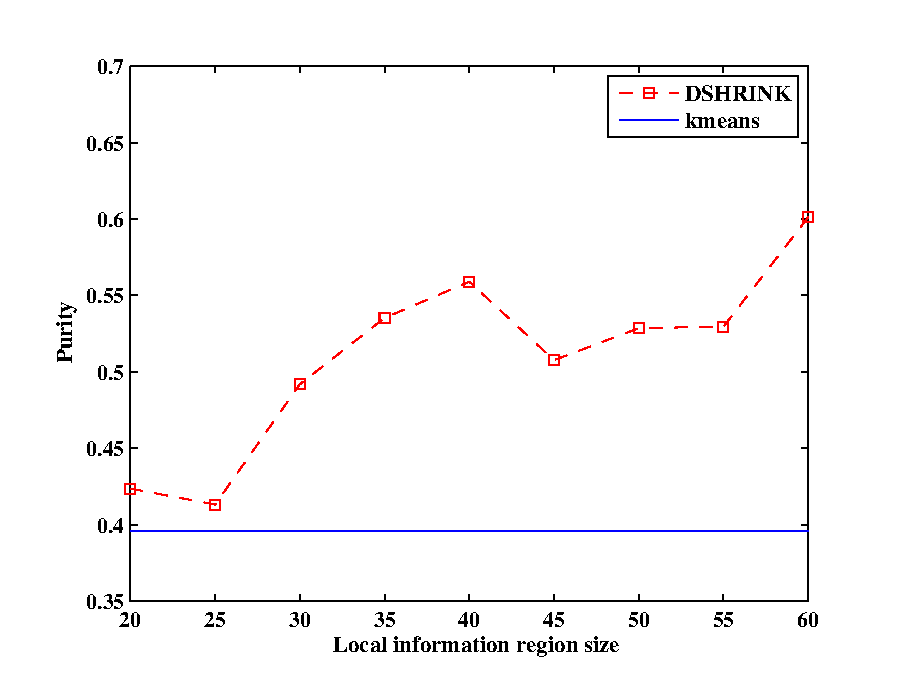
\includegraphics[width=1\textwidth]{chap2/blogcatalog_node_max}
    \caption{Blogcatalog-a在不同局部信息网络大小下的纯度}
    \label{fig:node_max:a}
\end{figure}

\begin{figure}
    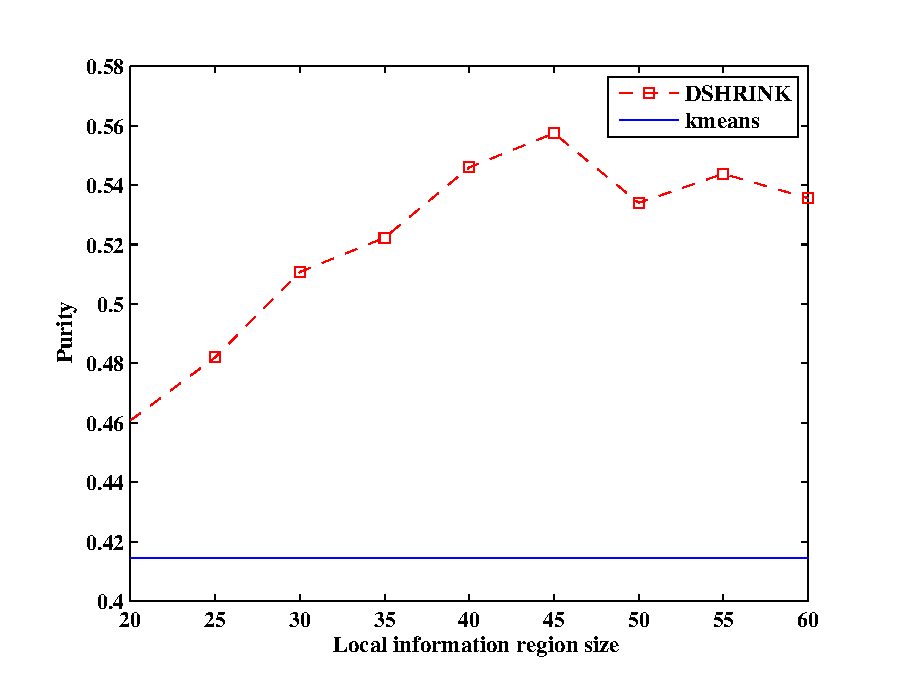
\includegraphics[width=1\textwidth]{chap2/blogcatalog_b_node_max}
    \caption{Blogcatalog-b在不同局部信息网络大小下的纯度}
    \label{fig:node_max:b}
\end{figure}

\subsection{不同的局部信息网络个数}
\label{sec:results_region_num}

在Blogcatalog-a和Blogcatalog-b做社区挖掘所得到的纯度随局部信息网络大小不同的变化如图\ref{fig:region_num:a}和图\ref{fig:region_num:b}。
此时选取的信息网络的大小为50。从实验结果可以看出,DSHRINK总是能比kmeans有更好的纯度,
同时总体的趋势是随着局部信息网络大小的增加,纯度变高。

\begin{figure}
    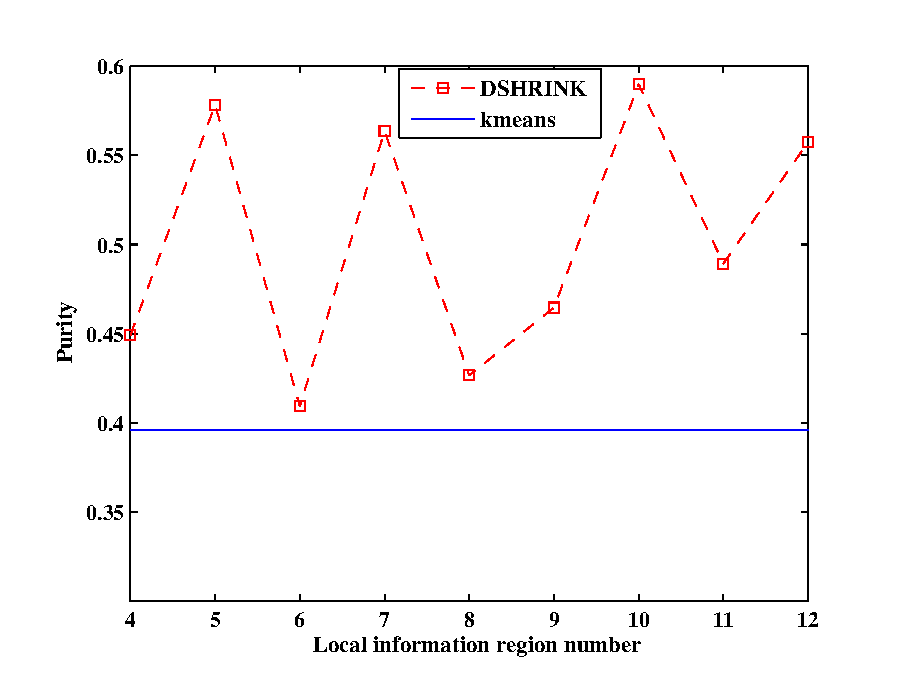
\includegraphics[width=1\textwidth]{chap2/blogcatalog_region_num}
    \caption{Blogcatalog-a在不同局部信息网络个数下的纯度}
    \label{fig:region_num:a}
\end{figure}

\begin{figure}
    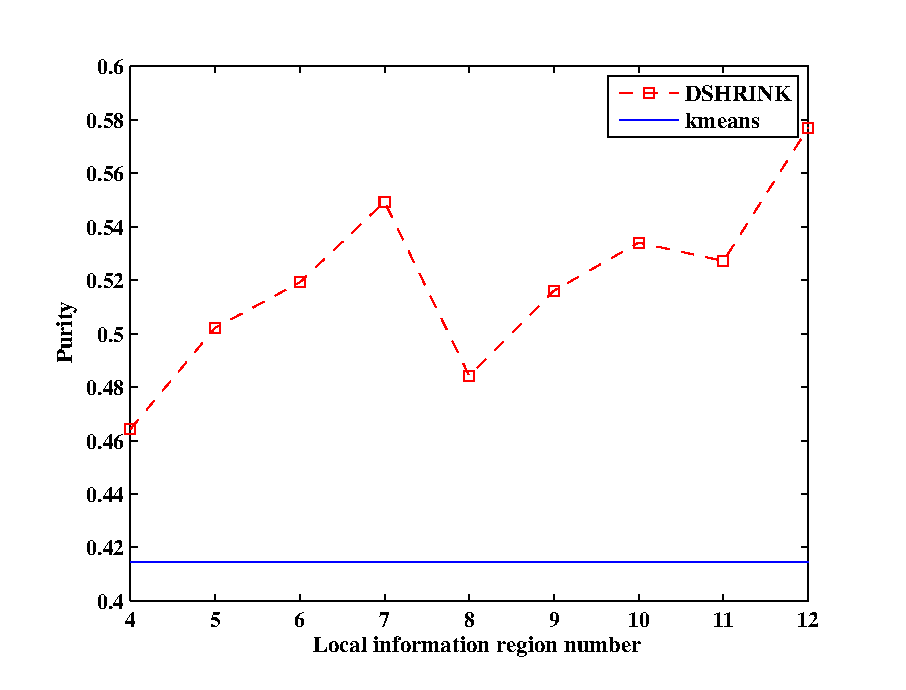
\includegraphics[width=1\textwidth]{chap2/blogcatalog_b_region_num}
    \caption{Blogcatalog-b在不同局部信息网络个数下的纯度}
    \label{fig:region_num:b}
\end{figure}

\subsection{实验结果分析}

DSHRINK相对于kmeans有更高的纯度是因为kmeans只是单纯地根据节点之间的欧式距离进行聚类,
而DSHRINK根据已知的信息在欧式距离的基础上进行了一定的调整,
这个距离能够保证相似的节点之间的距离更近,不相似的节点之间的距离更远。
基于这个距离对节点进行聚类,
能够达到更好的聚类效果。
而且,局部信息网络的个数越多或者局部信息网路的大小越大,知道的信息越多,
使用本文提到的算法进行聚类的纯度越高。

同时,DSHRINK聚类能够根据模块性准则自动地得到一个合适的聚类个数,而对于kmeans来说,
必须要先确定聚类的个数K才能聚类。对于实际的问题来说,聚类的个数是未知的,
此时如果要使用kmeans算法的,就必须尝试各种不同的k来确定达到一个比较好的聚类效果。
确定k的过程需要进行大量的实验,是一个十分耗时的过程。从这一点上,
本文算法具有相当大的优势。另外,从实验的过程中我们发现,
最终结果的好坏和选取的$\epsilon$没有关系,但是更大的$\epsilon$能够导致在每次迭代的过程中,有更多的节点被
合并到一个当地社区,因此能够减少迭代的次数,加快整个实验的运行。

\section{本章小节}

在本章中,我们详细阐述了实现本文算法实现时的实验环境与实验的各个步骤。
同时,通过对比本文算法和kmeans算法在不同的数据集和不同局部信息网络下的实验结果,
得出本文算法能够比kmeans算法在信息缺失的信息网络中具有更好地效果,
具有很好的实用性。

\chapter{本文总结}
\label{chap:summary}

\section{本文总结}

在本文中,我们实现了一种在信息缺失的社交网络中进行社区挖掘的算法,它使用了距离度量学习的概念,利用局部完整信息网络学习一个距离度量,然后基于这个距离进行聚类。
本文实现了整个过程,并在不断地试验中改进算法。
本文采用的数据集来自Blogcatalog,
从\ref{chap:result}可以看出解决, 本文的算法相对于K-means算法具有更高的精度,对于信息缺失网络下的社区挖掘具有更高的可靠性和实用性。

\section{存在的问题与解决方法}

\subsection{数据集的选取}

为完成本文的实验,选取的数据集必须要满足一下两个条件:

\begin{enumerate}
\item 挑选出合适的特征作为节点的属性
\item 节点之间存在边用于形成局部信息区域
\item 节点存在标签信息作为事实(Ground Truth)用于评价最后的结果
\end{enumerate}

为了得到这样的数据集,我们首先尝试使用新浪微博的数据进行实验,使用Python语言实现了一个爬取新浪微博数据的
\href{https://github.com/chouqin/weibo-crawler}{爬虫},
该爬虫能够爬取用户的微博,资料以及用户之间互相关注的信息。
同时,通过NLPIR分词库对用户的微博的进行分词,提取用户的关键字作为用户的属性。
但是由于新浪微博的限制,爬取大量用户的微博很难实现,而且新浪微博没有哪些用户的社区信息,
缺少这个信息就不能对算法进行评价,所以决定采取其他的数据集进行实验。

然后先后尝试了Google+, Facebook,Twitter的数据集,但都因为数据量不够而放弃使用。
接着又尝试了Flixter的数据集用于实验,可是它没有Ground Truth,只好放弃。最终选定了论文用于实验的Blogcatalog的数据集。

\subsection{信息缺失网络的构成}

由社交网络信息生产的数据集需要进行以下两个步骤才能转化为实验需要的信息缺失网络:

\begin{enumerate}
\item 由于从社交网络抓取到的数据比较多,需要抓取的数据集进行采样,选取适量个数的节点。
在选取的时候,利用节点的类信息,选取几个数目差不多的类,然后选取属于这几个类的节点作为样本。
具体的取样过程见\ref{sec:imple:dataset}
\end{enumerate}
\item 由于取样的数据集并不大,可以得到所有节点完整的信息。
为了得到一个信息缺失的网络,可以随机地生成几个局部信息网络,
然后只保留这几个局部信息网络的信息。生成局部信息网络的方法如下:
随机选取一个没有在任何局部信息网络中的节点,然后利用宽度优先搜索(Broad Frist Search, BFS)添加节点到当前的局部信息网络,
直到达到指定的个数为止。

\subsection{属性的选取}

在选取了特定的节点之后,要生成合适的属性信息用于计算节点之间的距离。
因为数据集中的节点的属性是稀疏的(也就是说,节点大部分的属性值都是0),
有必要对属性进行一定的处理。本文采用PCA进行特征提取。具体请看\ref{sec:imple:dataset}

\subsection{中间结果的验证}

因为整个算法分为两步,必须要确保第一步结果的正确才能开始第二步的实验。
为验证距离学习的正确性,对比谱聚类算法在第一步学习到的马氏距离和原来的欧式距离上的结果,
如果马氏距离的结果优于欧式距离,则说明第一步正确。

\subsection{DSHRINK算法的实现}

在用DSHRINK算法进行聚类时,发现聚类的结果不是很好,
一个经常出现的情况是大部分的节点都被聚到了一个聚类,
而其他聚类的节点个数则非常少,经过反复的实验,发现可以从以下几个方面进行改进:

\begin{enumerate}
\item 每次在挑选节点组成当地社区(Local community)时,对节点的所有近似最近节点按照和节点的距离进行排序,
然后按照距离从小到大进行选取。
\item 每次把一个local community合并成一个超级节点时,需要重新计算这个超级节点和其他节点之间的距离,
可以按照需要选取local community中所有节点距离的最小值,最大值和平均值作为超级节点的距离。
\end{enumerate}

\section{未来展望}

由于作者研究能力有限,经验不足,而且研究时间有限,本文提出的算法还有一些可以改善的空间:

首先,在数据选取方面,本文采用的两组实验数据都来自于Blogcatalog的数据集。如果具有更多的时间,仍然可以尝试使用其他的数据集进行实验。同时,在时间允许的情况下,本文实现的新浪微博爬虫也可以得到更多的改进,用于抓取有用的数据。

其次,在学习距离度量时,现在有很多的距离度量学习算法,本文选取了DCA算法用于学习距离度量,可以实现多种度量学习算法对比实验结果,然后选取其中最好的度量学习算法。

最后,在进行实验时,由于算法具有一定的随机性,对于不同的条件,重复执行5次求得实验结果。如果有足够的时间,应该重复更多的次数,这样结果会更加准确。

%%%==================================================
%% conclusion.tex for SJTU Master Thesis
%% based on CASthesis
%% modified by wei.jianwen@gmail.com
%% version: 0.3a
%% Encoding: UTF-8
%% last update: Dec 5th, 2010
%%==================================================

\chapter*{全文总结\markboth{全文总结}{}}
\addcontentsline{toc}{chapter}{全文总结}

这里是全文总结内容。

 %% 全文总结


%%%%%%%%%%%%%%%%%%%%%%%%%%%%%% 
%% 附录(章节编号重新计算,使用字母进行编号)
%%%%%%%%%%%%%%%%%%%%%%%%%%%%%% 
%\appendix

%% 附录中编号形式是"A-1"的样子
%\renewcommand\theequation{\Alph{chapter}--\arabic{equation}}
%\renewcommand\thefigure{\Alph{chapter}--\arabic{figure}}
%\renewcommand\thetable{\Alph{chapter}--\arabic{table}}

%%%==================================================
%% app1.tex for SJTU Master Thesis
%% based on CASthesis
%% modified by wei.jianwen@gmail.com
%% version: 0.3a
%% Encoding: UTF-8
%% last update: Dec 5th, 2010
%%==================================================

\chapter{模板更新记录}
\label{chap:updatelog}

\textbf{2012年12月21日} v0.5.1发布,在 \LaTeX 命令和中文字符之间留了空格,在Makefile中增加release功能。

\textbf{2012年12月5日} v0.5发布,修改说明文件的措辞,更正Makefile文件,使用metalog宏包替换xltxtra宏包,使用mathtools宏包替换amsmath宏包,移除了所有CJKtilde(\verb+~+)符号。

\textbf{2012年5月30日} v0.4发布,包含交大学士、硕士、博士学位论文模板。模板在\href{https://github.com/weijianwen/sjtu-thesis-template-latex}{github}上管理和更新。

\textbf{2010年12月5日} v0.3a发布,移植到 \XeTeX/\LaTeX 上。

\textbf{2009年12月25日} v0.2a发布,模板由CASthesis改名为sjtumaster。在diss.tex中可以方便地改变正文字号、切换但双面打印。增加了不编号的一章“全文总结”。
添加了可伸缩符号(等号、箭头)的例子,增加了长标题换行的例子。

\textbf{2009年11月20日} v0.1c发布,增加了Linux下使用ctex宏包的注意事项、.bib条目的规范要求,
修正了ctexbook与listings共同使用时的断页错误。

\textbf{2009年11月13日} v0.1b发布,完善了模板使用说明,增加了定理环境、并列子图、三线表格的例子。

\textbf{2009年11月12日} 上海交通大学硕士学位论文 \LaTeX 模板发布,版本0.1a。

 % 更新记录
%%% app2.tex for SJTU Master Thesis
%% based on CASthesis
%% modified by wei.jianwen@gmail.com
%% version: 0.3a
%% Encoding: UTF-8
%% last update: Dec 5th, 2010
%%==================================================

\chapter{Maxwell Equations}

选择二维情况,有如下的偏振矢量
\begin{subequations}
  \begin{eqnarray}
    {\bf E}&=&E_z(r,\theta)\hat{\bf z} \\
    {\bf H}&=&H_r(r,\theta))\hat{ \bf r}+H_\theta(r,\theta)\hat{\bm
      \theta}
  \end{eqnarray}
\end{subequations}
对上式求旋度
\begin{subequations}
  \begin{eqnarray}
    \nabla\times{\bf E}&=&\frac{1}{r}\frac{\partial E_z}{\partial\theta}{\hat{\bf r}}-\frac{\partial E_z}{\partial r}{\hat{\bm\theta}}\\
    \nabla\times{\bf H}&=&\left[\frac{1}{r}\frac{\partial}{\partial
        r}(rH_\theta)-\frac{1}{r}\frac{\partial
        H_r}{\partial\theta}\right]{\hat{\bf z}}
  \end{eqnarray}
\end{subequations}
因为在柱坐标系下,$\overline{\overline\mu}$是对角的,所以Maxwell方程组中电场$\bf
E$的旋度
\begin{subequations}
  \begin{eqnarray}
    &&\nabla\times{\bf E}=\mathbf{i}\omega{\bf B} \\
    &&\frac{1}{r}\frac{\partial E_z}{\partial\theta}{\hat{\bf
        r}}-\frac{\partial E_z}{\partial
      r}{\hat{\bm\theta}}=\mathbf{i}\omega\mu_rH_r{\hat{\bf r}}+\mathbf{i}\omega\mu_\theta
    H_\theta{\hat{\bm\theta}}
  \end{eqnarray}
\end{subequations}
所以$\bf H$的各个分量可以写为:
\begin{subequations}
  \begin{eqnarray}
    H_r=\frac{1}{\mathbf{i}\omega\mu_r}\frac{1}{r}\frac{\partial
      E_z}{\partial\theta } \\
    H_\theta=-\frac{1}{\mathbf{i}\omega\mu_\theta}\frac{\partial E_z}{\partial r}
  \end{eqnarray}
\end{subequations}
同样地,在柱坐标系下,$\overline{\overline\epsilon}$是对角的,所以Maxwell方程组中磁场$\bf
H$的旋度
\begin{subequations}
  \begin{eqnarray}
    &&\nabla\times{\bf H}=-\mathbf{i}\omega{\bf D}\\
    &&\left[\frac{1}{r}\frac{\partial}{\partial
        r}(rH_\theta)-\frac{1}{r}\frac{\partial
        H_r}{\partial\theta}\right]{\hat{\bf
        z}}=-\mathbf{i}\omega{\overline{\overline\epsilon}}{\bf
      E}=-\mathbf{i}\omega\epsilon_zE_z{\hat{\bf z}} \\
    &&\frac{1}{r}\frac{\partial}{\partial
      r}(rH_\theta)-\frac{1}{r}\frac{\partial
      H_r}{\partial\theta}=-\mathbf{i}\omega\epsilon_zE_z
  \end{eqnarray}
\end{subequations}
由此我们可以得到关于$E_z$的波函数方程:
\begin{eqnarray}
  \frac{1}{\mu_\theta\epsilon_z}\frac{1}{r}\frac{\partial}{\partial r}
  \left(r\frac{\partial E_z}{\partial r}\right)+
  \frac{1}{\mu_r\epsilon_z}\frac{1}{r^2}\frac{\partial^2E_z}{\partial\theta^2}
  +\omega^2 E_z=0
\end{eqnarray}
 % 麦克斯韦方程
% \include{body/app3}


%%%%%%%%%%%%%%%%%%%%%%%%%%%%%% 
%% 文后(无章节编号)
%%%%%%%%%%%%%%%%%%%%%%%%%%%%%% 
\backmatter

% 参考文献
% 使用 BibTeX
% 包含参考文献文件.bib
\bibliography{reference/chap1,reference/chap2}

% 致谢
%%==================================================
%% thanks.tex for SJTU Master Thesis
%% based on CASthesis
%% modified by wei.jianwen@gmail.com
%% version: 0.3a
%% Encoding: UTF-8
%% last update: Dec 5th, 2010
%%==================================================

\begin{thanks}

  感谢所有测试和使用交大硕士学位论文 \LaTeX 模板的同学!

  感谢那位最先制作出博士学位论文 \LaTeX 模板的交大物理系同学!

  感谢~William Wang~同学对模板移植做出的巨大贡献!

  感谢李奇平同学的使用!

  呵呵!

\end{thanks}
 

% 英文大摘要
\chapter{Community Detection in Incomplete Social Networks}
\label{chap:longabstract}

Communities in social networks are groups of users which are densely
connected inside the group, while loosely connected with nodes outside the group.
Users belong to one community tends to have much more in common, 
they may share some common interests or have some common properties.
Detecting communities in social communities is very import to analyze
social networks.

Detecting communities in incomplete social networks has two meanings.
First, detecting communities in social networks can be viewed as an clustering problem,
of which there are many existing algorithms; 
Second, when the social network is incomplete, that is, there are some information missing
in the social networks, the problem gets much more tough.
In this paper, we propose an algorithm that can detecting communities in incomplete social networks.

First, we identify and define the problem of incomplete networks.
Incomplete networks are information networks that have some information missing,
while there are many kinds of information missing regards to this problem,
in this paper, we deals with the incomplete information networks that still
has a few tiny local information regions. In these local regions, we can obtain
complete information of all nodes.

Second, we introduce a distance metric learning algorithm DCA to measure the 
distance between nodes in information networks. Using this distance metric,
we can compute the distance between any pair of nodes, which can reflect the
structural relation between nodes in incomplete networks. That is,
the distance between nodes that are similar to each other tends to be closer
than nodes that are dissimilar. To get such a distance metric, 
we turn the information in local information regions into 
contextual constraints which indicate the relevance relationship (positive or negative)
between nodes. The basic idea of DCA is to learn an
optimal data transformation that leads to the optimal distance 
metric by both maximizing the total variance between
the discriminative data chunklets and minimizing the total
variance of data instances in the same chunklets.

After such an distance metric has been learned, we can 
use some clustering algorithm to finish the community detecting process. 
In this paper, we propose a distance based clustering algorithm DSHRINK which can discover
the hierarchical communities. The DSHRINK clustering algorithm works as follows:
it iteratively combine nodes that are very closed to each other into one super nodes,
which can be combined in the next iteration. A distance based modularity function is devised
to evaluate the quality of the communities. Combination of low equality is stopped to 
get high purity of the clustering. We use this modularity to guide our clustering algorithm.
Moreover, so as to speedup the DSHRINK clustering process, we use an approximation strategy 
which leads to more nodes being combined during each iteration.

To evaluate the performance of our algorithm, we conduct a lot of experiments to compare
the purity of community detection using our methods and the kmeans clustering algorithm.
Empirical studies on real-world information networks show that our proposed
method can effectively detect community structures within incomplete social networks.

To conduct experiments, we first need to get proper datasets.
The datasets we choose must satisfy the following three conditions:
\begin{inparaenum}[i)]
    \item Each nodes must have proper attributes.
    \item There are some edges between nodes to generate local information regions.
    \item Each nodes must have class labels as ground truth to evaluate the result of community detection.
\end{inparaenum}
In order to get such datasets, we first implement an python crawler to 
crawl the data in the Weibo social networks. This crawler can get user's 
tweets, profiles, followers and fans. At the same time, we use The NLPIR to cut words
and extract keywords for each user, which can be used as attributes of an user.
But because the limitation of Weibo, we can't crawl enough user's information,
what's worse, most users in Weibo don't have class labels to use as ground truth.   
So we finally choose use data of Blogcatalog to do the experiments. 
PCA are used to reduce the dimension of attributes. Normalizing features
are required before doing PCA.
While the Weibo crawler we implemented can't be used to this project,
can be very helpful to get data for future work.

After proper datasets has been obtained, we need to generate contextual constraints 
to learn distance metric. To generate positive constraints, 
we use the structural similarity of nodes in the same local information regions.  
Local information regions are sampled using this procedure:
suppose we want to get regionNum local information regions, each local information has 
regionSize nodes, we first randomly pick one node as start node, then use BFS to include 
regionSize nodes from its neighbors, which is a local information region. The above procedure continues until we have sampled 
regionNum local information regions. Negative constraints are generated using 
randomly sampled regionNum times regionSize nodes.

After the above process, using DCA to learn a distance metric, followed by DSHRINK to clustering nodes 
based on the distance learned, we finish the whole procedure of our community detection method.
In order to measure the effectiveness of our method, we adopt purity to evaluate the quality of the 
communities generate by different approaches. The definition of purity is as follows:
each cluster is first assigned with the class that has the most nodes in the cluster as it's label,
number of nodes this label contains is the cluster's label count,
and purity is defined by the sum of all clusters' label count divided by total number of nodes, 
or more formally, in equation \ref{equa:purity}. Using this purity, 
we compare our methods with kmeans clustering algorithm using different datasets 
and under different conditions. Because of randomness of our method, 
the result of each run may be significantly different even under the same conditions.  
To overcome this randomness, each experiment is repeated 5 times and take the 
average result as the final result.
An automation script is implemented to execute this procedure automatically.  

From result section \ref{sec:results} we can see that the method we proposed in this paper
both have effectiveness and efficiency over kmeans.
This is because our method not only use nodes' attributes
to compute distance, but also use 
the information in local information region as side knowledge.
In the result we can see, 
the larger the local region information's size,
or the more the local region information's number,
the more side knowledge we can obtain,
which results in the higher purity.
What's more, 
our approach can automatically detect the appropriate number of cmmunities by minimizing the 
distance based modularity. Since the number of communities is unknown, 
kmeans method has great limitation because it must number of communities k must be known to
use kmeans clustering. Choose the appropriate k is an hard problem which needs a lot of more 
efforts. our method has great advantage for detecting communities than kmeans.

The method we propose to detecting communities in incomplete networks 
can not only be used in social networks, but also a wide range of domains.
For example, we can use our method to biological networks, publication networks,
terrorist-attack networks, food web, and so on. 
It is very interesting to analyze these networks using our method. 


\end{document}
